% !TeX spellcheck = en_US
\documentclass[12pt]{article}

% !TeX root = ../Rules.tex
% !TeX spellcheck = en_US

% This document is for Macro  \newcommand variables.

\newcommand{\leaguename}{RoboCup Humanoid Soccer League\xspace}
\newcommand{\leaguenameabbr}{HSL\xspace}
\newcommand{\GoalScoredDelay}{15}
\newcommand{\LeagueEmail}{Placeholder for LeagueEmail}

% Free Kick variables
\newcommand{\FreeKickTime}{30} % seconds to complete a free kick
\newcommand{\KickOffBallFreeTime}{10} % seconds after which ball is free during kick-off
% Free kick avoidance radius is defined as the center circle radius for each field size
% This means the same exclusion zone as during kick-off applies to all free kicks
% See field dimensions table in environment.tex for specific values
% \newcommand{\FreeKickRadius}{the center circle radius (see Table~\ref{tab:field_dim})}

% Penalty and timing variables
\newcommand{\StandardPenaltyTime}{30} % seconds
\newcommand{\StandardPenaltyIncrease}{15} % seconds added for each subsequent penalty
\newcommand{\ReadyDelayTime}{10} % seconds delay after whistle before GameController playing signal

% Game Stuck variables
\newcommand{\LocalGameStuckTime}{10} % seconds ball hasn't moved
\newcommand{\GlobalGameStuckTime}{30} % seconds no robot within proximity of ball
\newcommand{\GameStuckProximity}{1} % metres

% Penalty Kick variables
\newcommand{\PenaltyKickTime}{60} % seconds for penalty kick attempt
\newcommand{\PenaltyShootoutKickTime}{60} % seconds for shootout penalty kick

% Robot activity thresholds
\newcommand{\FallenRobotGetUpTime}{20} % seconds to start get-up
\newcommand{\FallenRobotGetUpAttempts}{3} % maximum get-up attempts
\newcommand{\FallenRobotGetUpAttemptsDisturbed}{4} % attempts if externally disturbed
\newcommand{\InactiveRobotTime}{10} % seconds before inactive penalty

% Ball holding variables
\newcommand{\BallHoldingTime}{5} % seconds for field players
\newcommand{\BallHoldingTimeGoalkeeper}{10} % seconds for goalkeeper in own penalty area

% Timeout variables
\newcommand{\TeamTimeoutDuration}{5} % minutes maximum
\newcommand{\TeamTimeoutReadyTime}{2} % minutes for other team to be ready

% Communication limits
\newcommand{\UDPPacketLimit}{12000} % packets per game
\newcommand{\UDPPacketSize}{512} % bytes
\newcommand{\UDPDebugPacketRate}{1} % packet per second per robot
\newcommand{\GameControllerPacketRate}{2} % packets per second

\input{common/dates}

\setcounter{secnumdepth}{4}

\usepackage{times,fullpage,xspace,fancyhdr,url,color}
\usepackage[pdftex]{graphicx}
\usepackage[pdftex,
            colorlinks=true,
            urlcolor=black,
            linkcolor=black,
            citecolor=black,
            bookmarksopen=false,
            bookmarksnumbered=true,
            pdfstartview=FitH]{hyperref}

\pdfcompresslevel=9

\hypersetup{
 pdftitle={\leaguename (\leaguenameabbr) Rule Book},
 pdfauthor={Technical Committee \leaguenameabbr},
}
\usepackage{microtype}
\usepackage[utf8]{inputenc}
\usepackage{amsmath}
\usepackage{xargs}
\usepackage[colorinlistoftodos,prependcaption,textsize=tiny]{todonotes}
\usepackage{siunitx}
\usepackage[capitalize,noabbrev]{cleveref}
\usepackage[official]{eurosym}
\usepackage[useregional]{datetime2}
\usepackage{subcaption}
\usepackage{enumitem}
\usepackage{xcolor}
\DTMlangsetup[en-GB]{ord=raise,monthyearsep={,\space}}

% modern and easy to use tables tblr
\usepackage{tabularray}

\newcommandx{\unsure}[2][1=]{\todo[linecolor=red,backgroundcolor=red!25,bordercolor=red,#1]{#2}}
\newcommandx{\change}[2][1=]{\todo[linecolor=blue,backgroundcolor=blue!25,bordercolor=blue,#1]{#2}}
\newcommandx{\info}[2][1=]{\todo[linecolor=green,backgroundcolor=green!25,bordercolor=green,#1]{#2}}
\newcommandx{\improvement}[2][1=]{\todo[linecolor=orange,backgroundcolor=orange!25,bordercolor=orange,#1]{#2}}

% comment 'disable' in to disable all the todo notes :)
\usepackage
[
%disable
]{todonotes}

\usepackage[theorems]{tcolorbox}
\newtcbtheorem[number within=section]{hintbox}{}%
{colback=red!10,colframe=red!45!black,fonttitle=\bfseries}{th}

\usepackage{tikz}
\usetikzlibrary{backgrounds,arrows,calc,math,positioning,shapes, decorations.markings,decorations.pathreplacing}

\usepackage{tikz-3dplot}

\usepackage{tocloft}
\cftsetindents{section}{0em}{2em}
\cftsetindents{subsection}{0em}{2em}
\renewcommand\cfttoctitlefont{\hfill\Large\bfseries}
\renewcommand\cftaftertoctitle{\hfill\mbox{}}

\sloppy
\newcommand{\ie}{\mbox{i.\,e.}\xspace}
\newcommand{\eg}{\mbox{e.\,g.}\xspace}
%\newcommand{\cf}{\mbox{cf.}\xspace}
\newcommand{\cf}{see\xspace}
% \newcommand{\comment}[1]{\marginpar{\pdfannot width 4in height .5in depth 8pt {/Subtype /Text /Contents (#1)}}}
\newcommand{\inparagraph}[1]{\paragraph{#1\hspace{-1em} }}


% some colors
\definecolor{orange}{rgb}{1,0.5,0}
\definecolor{red}{rgb}{1,0,0}
\definecolor{green}{rgb}{0,1,0}


%%%%%%%%%%%%%%%%%%% GENERAL SECTION NUMBERING %%%%%%%%%%%%%%%%%%%%%%%

% Section numbering formats
\renewcommand{\thesection}{\Roman{section}}
\renewcommand{\thesubsection}{\arabic{subsection}}
\renewcommand{\thesubsubsection}{\arabic{subsection}.\arabic{subsubsection}}

% Counter hierarchy (important!)
\makeatletter
\@addtoreset{subsection}{section}
\@addtoreset{subsubsection}{subsection}
\makeatother

% unnumbered subsection that is still listed in toc
\makeatletter
\newcommand{\subsectionNoNumber}[1]{%
  \subsection*{#1}%
  \phantomsection%
  \addcontentsline{toc}{subsection}{\protect\numberline{}#1}%
}
\makeatother


%%%%%%%%%%%%%%%%%%% SPECIFIC SECTION FORMAT %%%%%%%%%%%%%%%%%%%%%%%
% 
% Subdivision for the laws of the game:
%
%   \law{<N>}{<Title>}
%   \sublaw{<Title>}
%   \paragraph{<Title>}
%
% NOTE: the number <N> mus be fixed, e.g.,
%   \law{3}{My Big Law}
%

% width reserved for the law number in the TOC, adjust if necessary
\newlength{\lawnumwidth}
\setlength{\lawnumwidth}{2em}

% only for unique hyperlink targets; does not affect sectioning
\newcounter{lawtmp} 

\newcommand{\law}[2]{%
  \par\refstepcounter{lawtmp}% creates a unique anchor each time (for hyperlinks)
  \setcounter{subsection}{#1}%
  \setcounter{subsubsection}{1}%
  \renewcommand{\thelawtmp}{\thesubsection}
  \subsection*{§ #1\quad #2}% printed heading
  %\addcontentsline{toc}{subsection}{\protect\numberline{}§ #1\quad #2}
  \addcontentsline{toc}{subsection}{%
    \protect\numberline{}\makebox[2.5em][l]{§ #1} #2%
  }%
}

\newcommand{\sublaw}[1]{%
  \par\refstepcounter{lawtmp}% creates a unique anchor each time (for hyperlinks)
  \begingroup
    \renewcommand{\thelawtmp}{\thesubsubsection}%
    \renewcommand{\thesubsubsection}{§~\thesubsection.\arabic{subsubsection}}%
    \subsubsection{#1}%
  \endgroup
}

\renewcommand{\theparagraph}{§~\thesubsubsection.\arabic{paragraph}}%


% proper names for the \Cref and \cref

%\crefname{lawtmp}{Law}{Laws}
%\Crefname{lawtmp}{Law}{Laws}

% simply use Paragraph numbers
\crefname{lawtmp}{§}{§}
\Crefname{lawtmp}{§}{§}
\Crefname{paragraph}{}{}

%%%%%%%%%%%%%%%%%%% TEXT FORMAT %%%%%%%%%%%%%%%%%%%%%%%

\setlength{\parindent}{0pt}
\setlength{\parskip}{12pt plus 6pt minus 3 pt}
\widowpenalty=10000
\clubpenalty=10000

% needed to align an image and text correctly side by side
%\newcommand{\imagebox}[1]{\raisebox{2ex}{\raisebox{-\height}{#1}}}


%%%%%%%%%%%%%%%%%%% TITLE %%%%%%%%%%%%%%%%%%%%%%%

\title{Rule Book\\\leaguename (\leaguenameabbr)}

\author{\leaguename Technical Committee\\\url{https://hsl.robocup.org/}}
\date{(DRAFT \RCYear Working Rules Document, as of \today)}

\renewcommand{\headrulewidth}{0.4pt}
\renewcommand{\footrulewidth}{0.4pt}

%%%%%%%%%%%%%%%%%%% PAGE HEADER FORMAT %%%%%%%%%%%%%%%%%%%%%%%

\pagestyle{fancy}
% make sure that a separate page can be identified 
\lhead{Rule Book}
\chead{\leaguename}
\rhead{\today}
\lfoot{}
%\cfoot{}
%\cfoot{\thepage}
\rfoot{}


\begin{document}

\pagenumbering{Roman}

\maketitle
\thispagestyle{empty}

\begin{center}
  Questions or comments on these rules should be submitted via the following channels:
  \begin{itemize}
      \item \url{https://github.com/RoboCup-HumanoidSoccerLeague/HSL-Rules/issues};
      \item Discord server: \url{https://discord.gg/67upw6Nn}, channel \texttt{\#rule-book};
      \item Email:\footnote{a dedicated mailing list for the \leaguenameabbr will be set up and should be used in the future. For now any of the two mailing lists of the former leagues can be used.}
      \begin{itemize}
        \item (SPL) \url{rc-spl-tc-owner@lists.robocup.org}
        \item (HL) \url{rc-hl-tc@lists.robocup.org}
      \end{itemize}
  \end{itemize}
\end{center}

\newpage
\setcounter{tocdepth}{2}
\tableofcontents

\thispagestyle{fancy}

\clearpage
\pagenumbering{arabic}
\setcounter{page}{1}

\newpage

\include{rules/introduction}
\newpage

% !TeX root = ../Rules.tex
% !TeX spellcheck = en_US
\section{Notes and modifications}
\label{sec:modifications}

\subsectionNoNumber{Notes on the Laws of the Game}
\label{sec:notes_on_the_laws}

\subsectionNoNumber{Official Languages}

RoboCup Humanoid Soccer League Technical Committee publishes the Laws of the Game in English.

\subsectionNoNumber{Measurements}
If there is any divergence between metric and imperial units, the metric units are authoritative.

\subsectionNoNumber{Gender-Neutral Language}
References to human referees, assistant referees, and officials are formulated using gender-neutral language.
References to robot players use the neutral pronoun \emph{it} and \emph{its}. 

\subsectionNoNumber{General Modifications}
Subject to the agreement of the member association concerned and provided the principles of these Laws are maintained, 
the Laws may be modified in their application for regional matches.
Any or all of the following modifications are permissible:
\begin{itemize}
    \item size of the field of play
    \item size, weight and material of the ball
    \item width between the goalposts and height of the crossbar from the ground
    \item duration of the periods of play
    \item substitutions
\end{itemize}


\newpage

% !TeX root = ../Rules.tex
% !TeX spellcheck = en_US
\section{Laws of the Game}

\law{1}{The Field of Play}
\label{sec:field}

% ADDED BY REINALDO

The competition consists of three distinct divisions, categorized specifically by the maximum physical height and weight of the robotic platforms.

To ensure a fair and proportionate competitive environment, the field dimensions, number of players and ball size will vary to align with the specific requirements of each division (see \Cref{sec:divisions} for more details).

\sublaw{Field surface}
\label{sec:field_surface}

The matches are played on artificial turf with a height between approximately 20 to 30 mm, except for the small division, which has a height between 8 and 12 mm, also approximately.

The color of artificial turf must be green. No particular shade is required, but the green must contrast well with the field markings and the ball and should not be very dark.

\sublaw{Field markings}
\label{sec:field_markings}

The field of play must be rectangular and marked with continuous lines.
These lines belong to the areas of which they are boundaries.

The color of the field markings should be white, whether applied by tape, paint, or made from white turf.

The two longer boundary lines are called touchlines (or sidelines). The two shorter lines are called goal lines.
The field of play is divided into two halves by a halfway line, which joins the midpoints of the two touchlines.

A team's half is the half of the field that is closest to the team's own goal, where it primarily defends against opposing attacks.

The center mark is at the midpoint of the halfway line. A circle is marked around it, defining the center circle, a region used for kick-offs and other specific plays.

The goal area and the penalty area are defined using lines drawn at right angles to the goal line.

All lines must be of the same width, which must be between 5 and 12 cm.

\Cref{fig:field_line_names} shows the field markings with the lines and its names.

\begin{figure}[h]
    \centering
    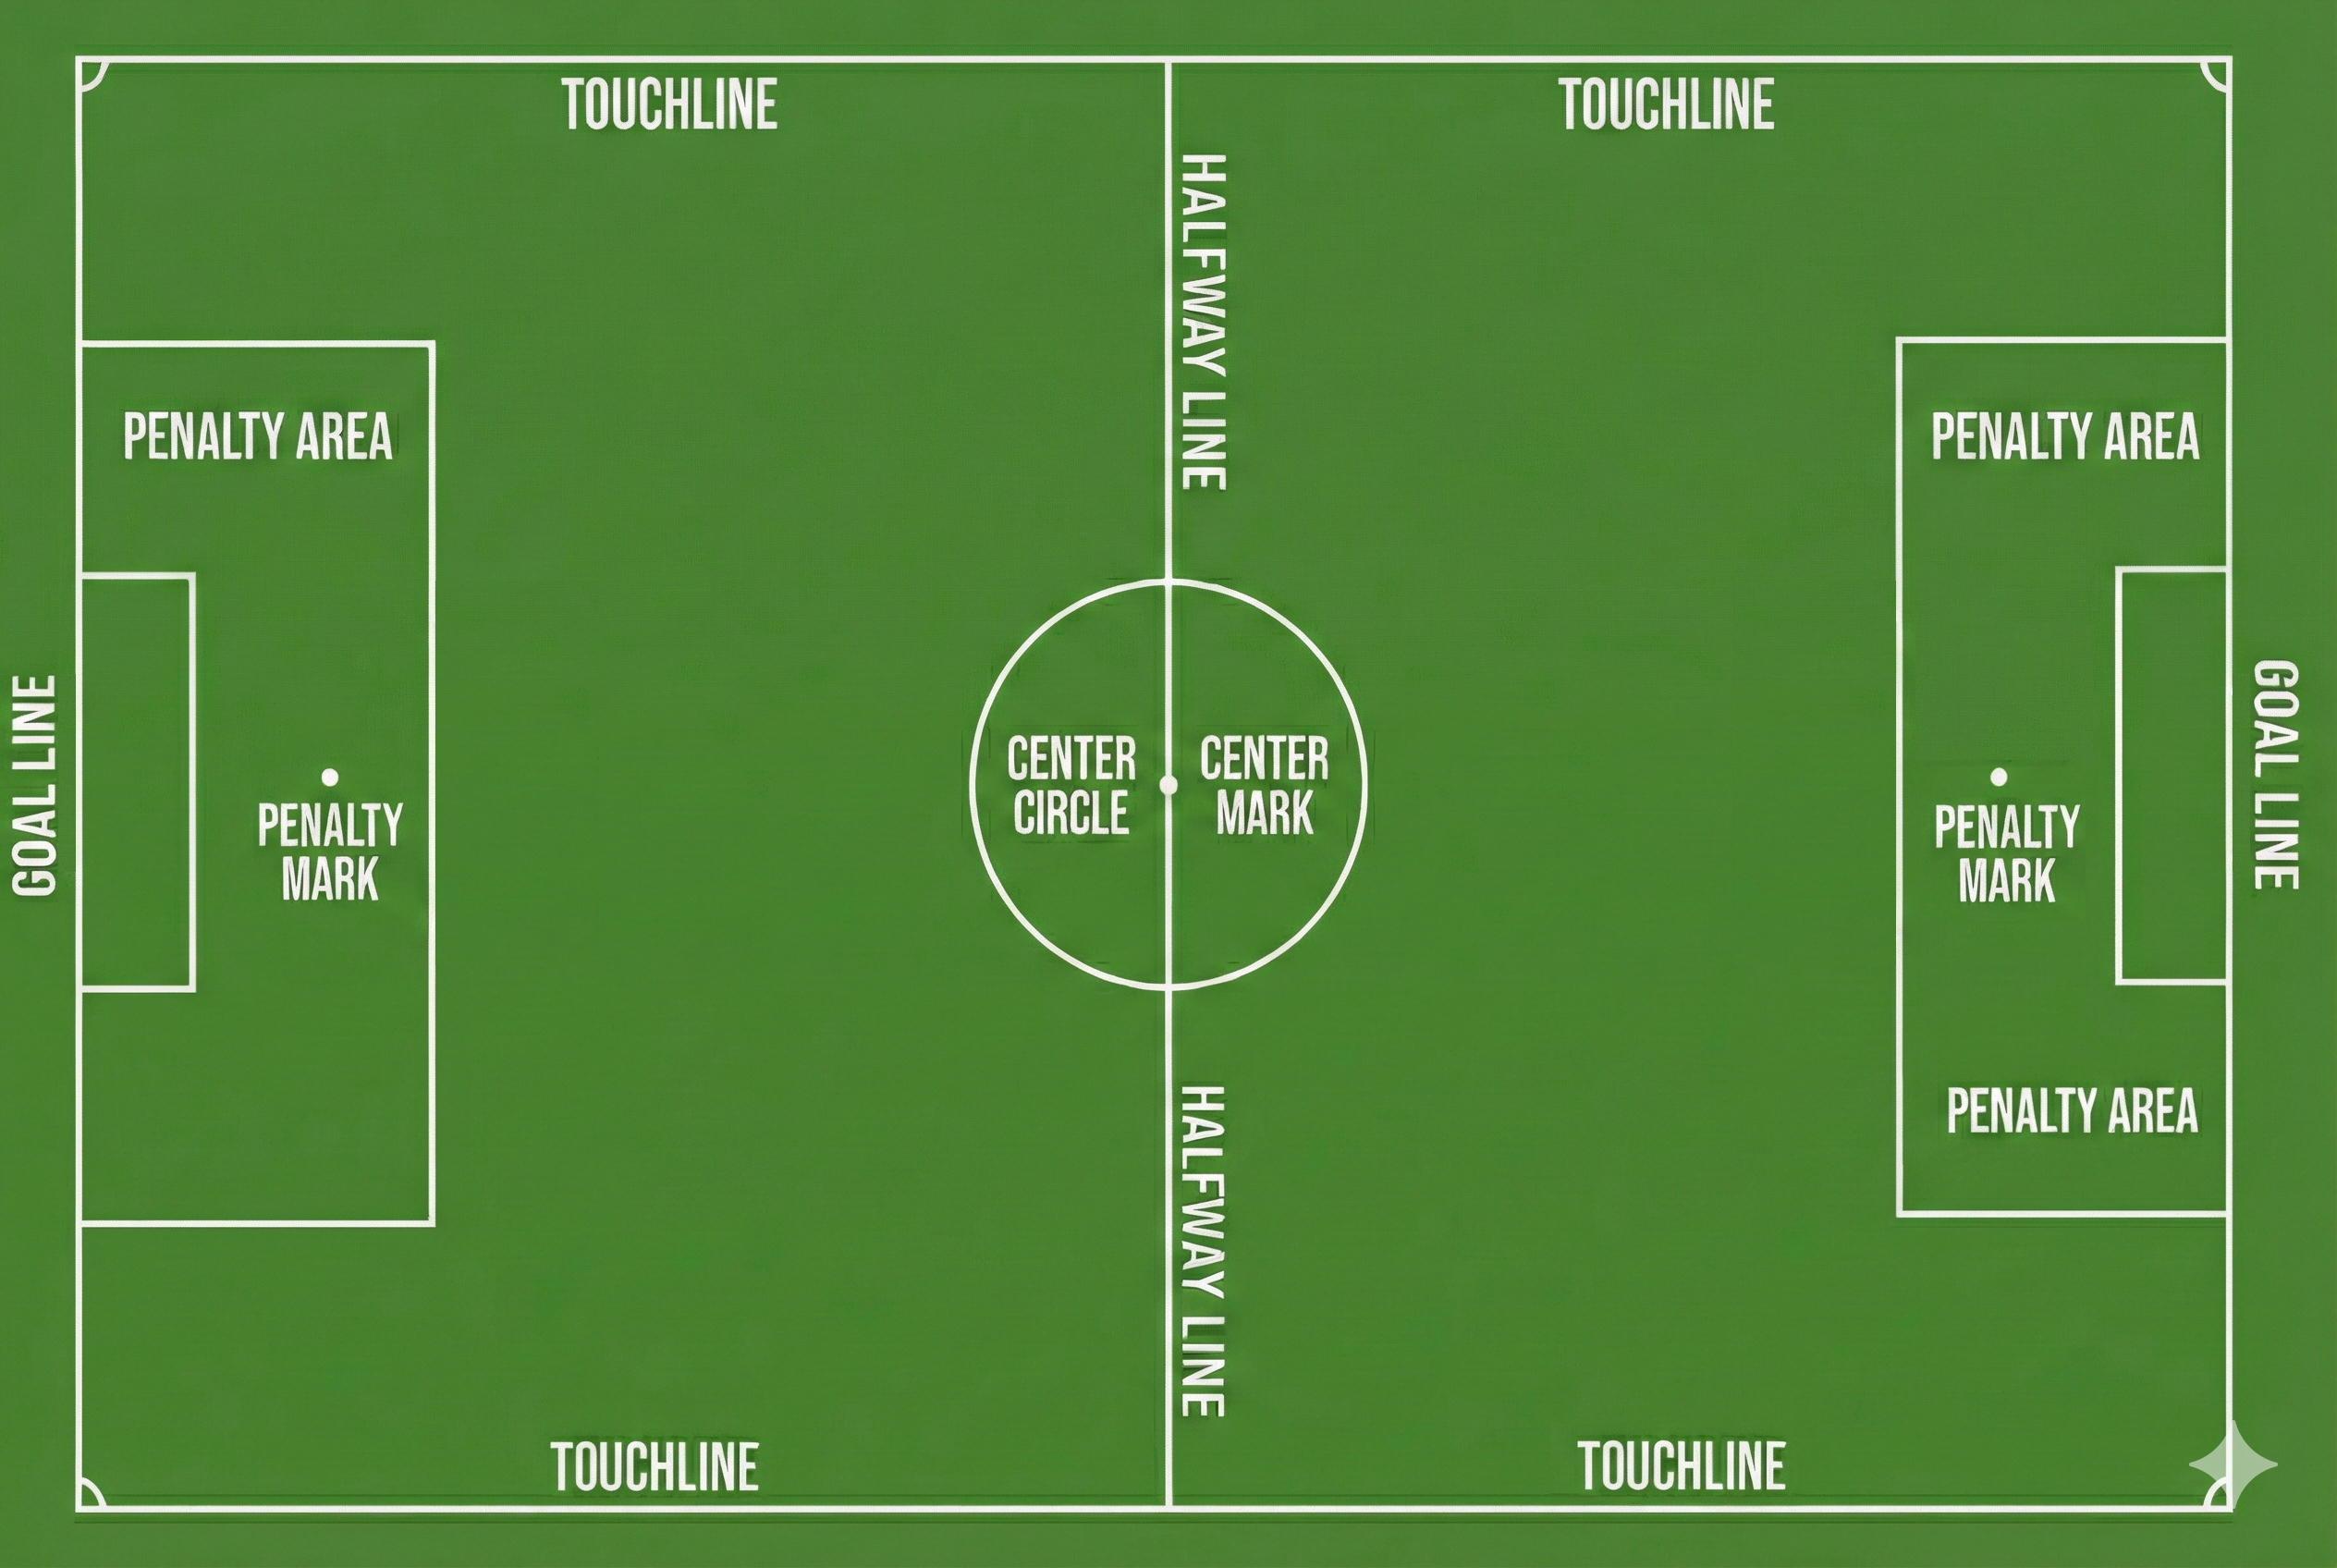
\includegraphics[width=0.7\columnwidth]{figs/Figure-1-line-names.png}
    \caption{Annotated diagram illustrating the standard markings and key areas of a soccer field.}      
    \label{fig:field_line_names}
\end{figure}

\sublaw{The goal area}
\label{sec:goal_area}

Two lines are drawn at right angles to the goal line; the length and distance from the midpoint of the goal line depend on the division.

These lines extend into the field of play and are joined by a line drawn parallel with the goal line.
The area bounded by these lines and the goal line is the goal area.

\sublaw{The penalty area}
\label{sec:penalty_area}

Two lines are drawn at right angles to the goal line; the length and distance from the midpoint of the goal line depend on the division.

These lines extend into the field of play and are joined by a line drawn parallel with the goal line.
The area bounded by these lines and the goal line is the penalty area. 

Within each penalty area, a penalty mark is made. 

\sublaw{The corner arc}
\label{sec:corner_arc}

A quarter circle from each corner is drawn inside the field of play.
The radius of the arc is 0.5m for the M-Field and 1.0m for the L-Field. The S-Field does not have corner arcs.

\sublaw{Dimensions}
\label{sec:dimensions}

There are three field sizes that can be used for the proposed divisions, described in \Cref{tab:field_dim_rule}.

\begin{table}[h]
    \centering
    \begin{tblr}{
        colspec = {X[l] X[c] X[c]},
        width=\linewidth,
        hlines,
        vlines,
        row{1} = {font=\bfseries}, % header
    }% begin tblr
        Field                  & Width (meters) & Length (meters) \\
        S-Field (small field)  & 6       & 9 \\
        M-Field (middle field) & 6 to 9  & 9 to 14 \\
        L-Field (large field)  & 9 to 14 & 14 to 22 \\
    \end{tblr}
    \caption{Approximate field sizes.}
    \label{tab:field_dim_rule}
\end{table}

\Cref{tab:field_dim} shows the dimensions of the S-, M- and L-Fields.
Diagrams of the three soccer fields are shown in \Cref{fig:field_small,fig:field_medium,fig:field_large}. 
Note that the Middle Division can be played on the S-Field or the M-Field, while the Large Division can be played on both the M-Field and the L-Field.
More detailed technical drawings are provided in \Cref{sec:technical_drawings}.

Note that measurements are from the outside of the lines as the lines are part of the area they enclose (as it is in the FIFA Rules).

\begin{table}[h]
    \centering
    \begin{tblr}{
        colspec = {c l X[c] X[c] X[c]},
        width=\linewidth,
        hlines,
        vlines,
        rows={f}, % align text in the middle 
        row{1} = {font=\bfseries}, % header
        row{2} = {font=\itshape}, % comments
        column{1} = {font=\bfseries}, % ids
    }% begin tblr
        ID & Description & S-Field  & M-Field  & L-Field \\
           & (all values in meters) & (former KidSize and SPL) & (former AdultSize) & (similar to MSL)\\

        A & Field length                 & 9.0 & 14.0 & 22.0 \\ 
        B & Field width                  & 6.0 & 9.0 & 14.0 \\ 
        C & Goal length (depth)          & 0.5 to 1.0 & 0.7 to 1.2 & 1.0 to 2.0 \\
        D & Goal width                   & 1.8 to 1.9 & 2.4 to 2.6 & 2.6 to 3.1 \\
        E & Goal Area length             & 1.0 & 1.0 & 1.0  \\ 
        F & Goal Area width              & 3.0 & 4.0 & 5.0  \\
        G & Penalty Area length          & 2.0 & 3.0 & 3.5  \\ 
        H & Penalty Area width           & 4.0 & 6.0 & 7.0  \\
        I & Penalty Mark distance        & 1.5 & 2.0 & 2.5  \\
        J & Center Circle diameter       & 1.5 & 3.0 & 4.0 \\
        K & Border strip width (min.)    & \SetCell[c=3]{c} 1.0 & & \\ 
        L & Corner Arc radius            & none & 0.5 & 1.0 \\ 
          & Line width                   & \SetCell[c=2]{c} 0.05 & & 0.12 \\
          & Penalty and center mark size & \SetCell[c=2]{c} 0.10 & & 0.15 \\
    \end{tblr}
    \caption{Exemplary field dimensions by field type, in meters.}   
    \label{tab:field_dim}
\end{table}


\begin{figure}[h]
  \centering
  \input{rules/small_field}
  \caption{Schematic diagram of the small soccer field -- S-Field (scale: 1/80)}
  \label{fig:field_small}
\end{figure}

\begin{figure}[h]
  \centering
  \input{rules/medium_field}
  \caption{Schematic diagram of the medium soccer field -- M-Field (scale: 1/100)}
  \label{fig:field_medium}
\end{figure}

\begin{figure}[h]
  \centering
 \input{rules/large_field}
  \caption{Schematic diagram of the large soccer field -- L-Field (scale: 1/150)}
  \label{fig:field_large}
\end{figure}

\sublaw{Goals}
\label{sec:goals}
A goal must be placed on the center of each goal line. 
A goal consists of two vertical posts equidistant from the corners and joined at the top by a horizontal crossbar. 

The goalposts and crossbar must be made of wood, metal, or other approved material and must not be dangerous to the players.

The goalposts and crossbar of both goals must be of the same shape, which must be square, rectangular, round, elliptical, or a hybrid of these options.\info{need a figure how goalposts must be placed on the goal line}

The goalposts and crossbar must have the same width, which is not less than 7 cm and does not exceed 12 cm.
The goalposts and the crossbar must be white. Goal nets and any net supports may be white, gray, or black.

Goals must be anchored securely to the ground. 

Off-the-shelf goals may be used if they satisfy these requirements. 


    

\begin{table}[h]
    \centering
    \begin{tblr}{
        colspec = {X[l] X[c] X[c] X[c]},
        width=\linewidth,
        hlines,
        vlines,
        row{1} = {font=\bfseries}, % header
    }% begin tblr
        Division & Width (meters) & Height (meters) & Depth (meters)\\
        Small    & 1.8 to 1.9 & 1.2 to 1.3 & 0.5 to 1.0 \\
        Middle   & 2.4 to 2.6 & 1.5 to 1.9 & 0.7 to 1.2\\
        Large    & 2.6 to 3.1 & 1.8 to 2.0 & 1.0 to 2.0\\
    \end{tblr}
    \caption{Allowed ranges for goal dimensions.}
    \label{tab:goal_dim}
\end{table}

\sublaw{Definition of Inside and Outside}

\label{sec:inside_outside}
An object (such as a {\color{red} robot} or the ball) \unsure{TW: are there other objects? if not why mentioned this?} is considered \textit{inside} a region of the field if any part of it overlaps or touches the boundary lines that define that region, or if it is fully contained within the region, in the air or on the ground. It is considered \textit{outside} the region only when no part of it, or its downwards projection, remains within or on the boundary lines of that region. This definition applies to any designated area of the field, except the goal (see \Cref{fig:field_line_names}).

\textbf{Exception for the goal:} The ball is only considered \textit{inside} the goal (and thus a goal is scored) if, and only if, the entire ball has wholly crossed the goal-side edge of the goal line \emph{between the goal posts and below the crossbar}, \ie{} when no part of the ball remains on or above the goal line, and the entire ball is within the volume enclosed by the goal frame and the net.
\improvement{TW: This needs to be discussed for robots.}

\improvement{TW: This definition, \textit{for robots} is inconsistent with former-SPL rules. I am unsure about former-HL. Robots are defined as inside/outside an area based on the feet touching (or body touching). The projection of the body has implications for illegal positioning, etc. This also has implications if a robot is "in the air". We haven't seen jumping robots yet.}

\improvement{TW: The terms inside/outside appear to be repeatedly redefined in various places. All should refer back to this section.}

\textbf{Exception for the Goal:} The ball is only considered \textit{inside} the goal (and thus a goal is scored) when the entire ball has wholly crossed the goal-side edge of the goal line, \ie{}, when no part of the ball remains on or above the goal line and the ball is outside the field of play.

\sublaw{Venue Setup}
\label{sec:venue_setup}

Fields may be located close to one another.
Barriers will not necessarily be constructed between adjacent fields to block the robots from seeing other fields, goals, or balls. 
However, barriers will be constructed to block sight between any fields that are not located at least three meters apart.
Hence, for each side of a field that is adjacent to another field, either barriers will separate the fields or at least \qty{3}{\metre} will be between the carpet of adjacent fields.

\sublaw{Lighting Conditions}
\label{sec:lightingConditions}

The \leaguenameabbr does not mandate specific or controlled lighting conditions for a match venue. It is expected that the venue provides reasonable lighting suitable for general visibility (\eg indoor with artificial lighting, outdoor with natural lighting, or a combination of both). 

The lighting conditions depend on the actual venue. Fields should be placed near or under windows where possible. 

Whether window lighting is used or not, ceiling lights should be provided as necessary so that most of the field is at least \qty{300}{\lux} (preferably \qty{400}{\lux}). This lighting may include variations such as glare, brightness, shadows, or mixed lighting conditions that can change throughout the match. 

However, the lighting must be predominantly white, and colored lighting that significantly changes the perceived color of the field or ball is not allowed. 

Teams participating in the \leaguenameabbr are encouraged to design their robots to handle a variety of typical lighting environments that may be encountered during a match. Natural and non-natural light must be free to reach the field. The technical committee can delimit a zone near the field where humans must not stand and where any items blocking the light sources are forbidden.

\law{2}{The Ball}
\label{sec:ball}

\sublaw{Qualities and measurements}
\label{sec:ball-measurements}

All balls must be spherical, made of or resembles the weight, form, movement characteristics and appearance of leather or other suitable material.

The balls for each division\footnote{The TC and OC will decide on only one type of the ball per division that will be used by all teams during the 2026 competition.} are defined in \Cref{tab:balls}.

    

\begin{table}[h]
    \centering
    \begin{tblr}{
        colspec = {X[l] X[l]},
        width=\linewidth,
        hlines,
        vlines,
        row{1} = {font=\bfseries}, % header
    }% begin tblr
        Division & Ball Type\\
        Small    & FIFA Mini Ball\\
        Middle   & FIFA size 3 or 4\\
        Large    & FIFA size 5 \\
    \end{tblr}
    \caption{Balls used in each division}
    \label{tab:balls}
\end{table}


\sublaw{Replacement of a defective ball}

If the ball bursts or becomes defective during the course of a match: the match is stopped. It is is restarted by dropping the replacement ball at the place where the original ball became defective.

If the ball bursts or becomes defective whilst not in play at a kick-off, goal kick, corner kick, free kick, penalty kick or throw-in: the match is restarted accordingly.

If the ball becomes defective during a penalty kick or penalties (penalty shoot-out) as it moves forward and before it touches a player, crossbar or goalposts, the penalty kick is retaken.

The ball may not be changed during the match without the referee’s permission.

\sublaw{Additional balls}
Additional balls which meet the requirements of \Cref{sec:ball-measurements} may be placed around the field of play and their use is under the referee's control.
\newpage

% !TeX root = ../Rules.tex
% !TeX spellcheck = en_US
\law{3}{Teams and Players}
\label{sec:teams_and_players}

\sublaw{Divisions and Configurations}
\label{sec:divisions}

A team belongs to one division, which is one of Small, Middle and Large. Main competition matches only take place between members in the same division.

Teams in each division can choose to play in two team configurations: Foundation - with a smaller number of players; and Advanced - with a larger number of players. If in a game one of the teams chooses to play in a Foundation configuration, then both teams must play in this configuration to ensure fairness. The maximum number of players in a game for each configuration is shown in Table \ref{tab:number_of_players}.

In the Middle division, starting from the quarter-finals onwards, all matches will be played in the Advanced configuration.

The division and the configuration preference of a team must be submitted before the competition. The division must not change during the competition itself.
The division must be submitted at the time of team registration. In addition, each team shall submit its preferred configuration prior to the competition, by a deadline specified by the organizers, in order to enable proper field planning.
A team may request to play in a different configuration during the competition by submitting a request to the organizers. Approval of such a request is at the sole discretion of the organizers.

\sublaw{Number of Players}
\label{sec:number_of_players}
A match is played by two teams, each with a \textbf{maximum} number of players determined by the division the game takes place in and the configuration level of the playing teams, as illustrated by the following table:

\begin{table}[h]
    \centering
    \begin{tblr}{
        colspec = {X[l] X[c] X[c]},
        width=\linewidth,
        hlines,
        vlines,
        row{1} = {font=\bfseries}, % header
    }% begin tblr
        Division & Foundation teams & Advanced teams\\
        Small & 4 & 7 \\
        Mid   & 3 & 5 \\
        Large & 3 & 5 \\
    \end{tblr}
    \caption{Number of players}
    \label{tab:number_of_players}
\end{table}

At most one player per team on the field may be designated as \emph{goalkeeper}, the others are all \emph{field players}.
When playing at full strength, a team must have a \emph{goalkeeper} on the field.

\sublaw{Number of Substitutes}
\label{sec:number_of_substitutes}
In addition, each team may prepare \emph{substitute players} outside the field. The number of substitute players is not limited.
A \emph{substitute player} may be substituted in to become a \emph{field player} or \emph{goalkeeper}.

\sublaw{Substitution Procedure}
\label{sec:substitution_procedure}
In all matches, the jersey numbers of the substitutes must be given to the referee prior to the start of the match. Any substitute whose jersey number is not given to the referee at this time may not take part in the match.

To replace a player with a substitute, the following conditions must be observed:
\begin{itemize}
  \item The referee must be informed before any proposed substitution is made.
  \item The substitution may only occur during a stoppage in the match.
  \item The player being replaced must first be removed from the field.
  \item The substitute only enters the field of play after the player being replaced has left and after receiving a signal from the referee.
  \item The substitute enters the field of play at the standard re-entry point (on the touchline at the height of the penalty mark in the robot's own half, as used for returning from a penalty).
  \item The substitution is completed when the substitute enters the field of play.
  \item From that moment, the substitute becomes a player and the player replaced becomes a substituted player.
  \item All substitutes are subject to the authority and jurisdiction of the referee, whether called upon to play or not.
\end{itemize}

\paragraph{Changing the Goalkeeper}

Any of the other players may change places with the goalkeeper, provided that:
\begin{itemize}
  \item The referee is informed before the change is made.
  \item The change is requested during a stoppage in the match.
\end{itemize}

\sublaw{Robot Players}
\label{sec:robot_players}

\paragraph{The Design of the Robots}
\label{sec:design_of_robots}
Robots participating in the \leaguenameabbr must have a human-like body shape with a torso, head, two arms, and two legs, as well as human-like symmetry and proportions regarding sizes of the body parts and weight distribution.

The robots must be able to stand upright on their feet, to walk on their legs and to be able to recover from a fall (get back to a standing position). 

The only allowed modes of locomotion are bipedal walking, running, and jumping. Soccer related movements such as dribbling, kicking, or other forms of ball handling are also allowed.

The design of the robot's arms, including their length and placement, shall permit arm use and behaviors that are reasonably comparable to those of humans. Examples of permitted uses include assisting in getting up after a fall or picking up and throwing the ball (where otherwise allowed by the rules).

Arm configurations that enable behaviors significantly different from those of humans are not permitted. In particular, 
robots must not use their arms to provide continuous support for locomotion, such as walking on arms or using arms as additional legs.

\paragraph{Size Restrictions}

All robots participating in the \leaguenameabbr must comply with the following restrictions:

The length of the legs $H_{leg}$, including the feet, satisfies 0.35{\textperiodcentered}$H_{top}$ ${\leq}$ $H_{leg}$ ${\leq}$ 0.7{\textperiodcentered}$H_{top}$,  where $H_{top}$ is the height of the top of the robot. 
The length of the leg is measured from the first rotating joint where its axis lies in the plane parallel to the standing ground to the tip of the foot.

A classic piece of human anatomy and art history, Leonardo da Vinci’s “Vitruvian Man” famously depicts a man whose arm span is equal to his height, creating a 1:1 ratio. 
Therefore, the arm span, $A_{span}$, including the hands, should satisfy 0.8{\textperiodcentered}$H_{top}$ ${\leq}$ $A_{span}$ ${\leq}$ 1.2{\textperiodcentered}$H_{top}$.

Based on $H_{top}$, the following size restrictions apply for each division:
%
\begin{itemize}
\item Small:  $H_{top}$ ${\leq}$ 1.1 meters;
\item Middle: $H_{top}$ ${\leq}$ 1.25 meters;
\item Large:  $H_{top}$ ${\leq}$ 1.9 meters.
\end{itemize}

$H_{top}$ is defined as the height of the robot when standing upright (with fully extended knees).
$H_{top}$ is measured with the head of the robot oriented in such a way that it
is tilted to either its maximum upwards tilt angle or the horizon line,
whichever is lower.

The height of the head $H_{head}$, including the neck, satisfies $0.1 \cdot H_{top} \leq H_{head} \leq 0.3 \cdot H_{top}$. $H_{head}$ is defined as the vertical distance from the axis of the first arm joint at the shoulder to the top of the head.

\paragraph{Weight Restrictions}

The robot's Body-Mass Index (BMI) is defined as follows:
$\mathrm{BMI} = \frac{M}{{H_{top}}^2}$,
where $M$ is the mass of the robot in kg and $H_{top}$ its height in meters.

The Body Mass Index (BMI) of the robot should be: $5 \leq \mathrm{BMI} \leq 30$.

The following weight restrictions apply for each division:
%
\begin{itemize}
\item Small:  Weight${\leq}$ 15 kilograms;
\item Middle: Weight ${\leq}$ 25 kilograms;
\item Large:  Weight ${\leq}$ 80 kilograms.
\end{itemize}

\paragraph{Safety}

A player must not use equipment or wear anything that is dangerous to himself or another player.

Robots are encouraged to be equipped with an emergency stop button that makes the robot immediately desist with all motions, 
or ideally go limp and/or cut power to the actuators. 

Robot operators must be able to immediately bring a robot to a safe state. 
The mechanism used to do this (e.g. emergency button on the robot, remote emergency button) is secondary. 
Most important is that robot operators are able to bring a robot to a safe state in an emergency.

Robot handlers are allowed to carry an additional remote emergency stop button.
This button must be worn either around the neck or on the belt of the robot handler and must be clearly marked. 
Each emergency stop button can only be connected to the robot of the robot handler that holds the button.
The remote emergency button cannot perform any additional functions. 
Robot handlers must keep their hands clearly away from the button unless the button is actively being pressed. 
Robot handlers must not use the remote emergency button to intentionally incapacitate their robots.

\improvement[inline]{to be discussed, add additional GameController based mechanism to immediately stop all robots, for example by setting an emergency stop game state}

\label{sec:design_of_robots}

\sublaw{Approved Standard Platforms}
The following commercially available robotic platforms are approved for participation in the \leaguenameabbr. 

The following are the list of pre-approved standard platforms that require no modifications:

\begin{tblr}{
  width=1.0\linewidth,
  colspec = {Q[l]Q[l]X[l]},
  row{1}={fg=black, font=\bfseries}, %, 
  hline{2} = {solid},
  hline{3-Y} = {dashed},
  vline{2,3} = {abovepos = -1, belowpos = -1},
}
Manufacturer & Model & Restrictions\\
%
Aldebaran & Nao V5, and Nao V6 \\
Robotis   & DARwIn-OP \\
Booster   & T1, and K1 \\
Fourier   & GR1, GR1-Pro, and GR2 \\
Unitiree  & G1++, H1++ \\
\end{tblr}

Additional humanoid robot platforms can be approved upon request. Please send your request for approval to \url{rc-spl-tc@lists.robocup.org}. \improvement{Change to new mailing list when ready}

\sublaw{Hardware}
\label{sec:hardware}

Modifications or additions to the robot hardware are permitted as long as the resulting robot does not become non-compliant with these rules.

No additional hardware is permitted, including off-board sensing or processing systems.
Additional sensors besides those originally installed on the robots are likewise not allowed.

\sublaw{Sensors}
\label{sec:sensors}

Teams participating in the \leaguenameabbr competitions are encouraged to equip their robots with sensors that have an equivalent in human senses. 
These sensors must be placed at a position roughly equivalent to the location of the human's biological sensors.

The sensors and their placement shall be chosen such that they allow the robot a spatial perception similar to humans.
%
The sensors are evaluated along the following two general guidelines:
\begin{enumerate}
    \item \emph{Foster and encourage research and development towards human-like perception capabilities.}\\
    Sensors aiming to directly emulate human senses, like a camera or a microphone. Use of such sensors is explicitly \emph{encouraged}.
    \item \emph{Enable research and development under the constraints of the current state of the art in technology and research, as long as this does not undermine current research efforts as declared in point 1.} \\
    Sensors that compensate for current shortcomings in technology and state of research, like one-dimensional distance sensors with limited range, or two vertically arranged cameras in the robot NAO.
\end{enumerate}

Generally, \emph{passive sensors} are preferred to \emph{active} sensors that actively emit signals.

\paragraph{Intrinsic Perception and Proprioception}
Any sensing capability aiming at measuring the internal state of the robot is permitted. 
This includes temperature, current consumed by the motors, joint positions, etc.

\paragraph{Visual Perception}
The visual sensors, e.g., cameras of the robot shall be arranged such that the combined visual field is \emph{contiguous} and limited to dimensions similar to a human, which corresponds to limitations in the opening angle: horizontal $\leq$ \SI{220}{\degree} and vertical $\leq$ \SI{160}{\degree}. 
Please note that these ranges may be adjusted to more human-like viewing angles in the future.

The visual sensors shall be located in the head of the robot.

The combined dynamic visual field that can be observed by the robot solely by moving its cameras (similar to human eye movements) and the head is limited to horizontal $\leq$ \SI{340}{\degree} and vertical $\leq$ \SI{220}{\degree}.

The cameras are restricted to visual information in the range of the light visible to humans.

The cameras can provide dense visual information, such as a rasterized image, or sparse information, such as visual events (event cameras).


\paragraph{Visual (dense) Depth Perception}

Passive integrated devices that provide dense depth information, such as stereo cameras, are permitted and encouraged.

Active integrated devices that provide depth information, such as cameras with an active infrared projector or time-of-flight cameras, are permitted but discouraged.
Their use might be prohibited in the future.


\paragraph{Orientation}

Sensors providing information regarding the robot's orientation in space with relation to the ground are permitted. This includes sensors such as gyrometer, accelerometer, as well as integrated inertial measurement units (IMU), as long as they provide only relative measurements and no measurements of the absolute direction, such as a compass.

An IMU with an integrated compass can be used as long as the compass not used.

The sensors can be placed in the head and/or in the torso of the robot.

\paragraph{Sound Perception}
The sound sensors, e.g., microphones, shall be placed in the head of the robot.
The number of microphones is not limited.

\paragraph{Haptic Sensing}
Any passive sensor allowing haptic measurement is permitted, such as force sensors, touch sensors, buttons/bumpers, capacitative touch sensors.

Haptic sensors can be placed at any location of the robot's body and are not limited in number.


\paragraph{Distance Sensing}

Active and passive sensors for one-dimensional distance sensing with a limited range are permitted if their use is limited to compensate for shortcomings in the spatial awareness of the robot in the close proximity.

%The range is limited to ...
The number of such distance sensors is limited to 4.

The use of distance sensors is discouraged and might be prohibited in the future.

\paragraph{Summary}
The following table briefly summarizes pre-approved sensors.
The use of listed sensors that are considered human-like is encouraged.
The use of listed sensors that are not considered human-like is accepted, but discouraged and might be prohibited or limited in the future.

\begin{tblr}{
  width=1.0\linewidth,
  colspec = {Q[l]Q[l]X[l]},
  row{1}={fg=black, font=\bfseries}, %, 
  hline{2} = {solid},
  hline{3-Y} = {dashed},
  vline{2,3} = {abovepos = -1, belowpos = -1},
}
Sensor Type & Human-Like & Comments \\

%Visual Perception
RGB camera & yes & opening angle limit: horizontal $\leq$ \SI{180}{\degree}, vertical $\leq$ \SI{140}{\degree}\\
Stereo camera & yes & \\
Event camera & yes & \\

Active RGB-D based on infrared projection & no & discouraged\\
Active RGB-D based on time of flight (TOF) & no & discouraged\\

% sound perception
Microphone array & yes & \\

% Orientation
Gyro & yes & \\
Accelerometer & yes & \\
Compass & no & magnetic measurement sensors are not allowed\\ 
Integrated inertial measurement units (IMU) & yes & no compass or must be disabled and not used\\

% Haptic sensing
Force sensors & yes & \\
Touch sensors & yes & \\
Buttons / Bumpers & yes & \\
Capacitive touch sensors & yes & \\

% Distance sensing
Near range infrared sensor & no & \\
Sonar / ultrasound sensors & no & \\
1D LIDAR and laser range sensor & no & with limited range \\

% Intrinsic sensors
Intrinsic sensors  & yes & temperature, current, joint positions, etc. \\
\end{tblr}

\sublaw{Communication}
\label{sec:communication}

Robots participating in the \leaguenameabbr competitions must act autonomously during a game. 

Any use external power supply, teleoperation, remote control, remote processing, remote sensing, or remote brain of any kind is prohibited.

Communication is only allowed among robots on the field, between the robots and the referees, and between the robots and the GameController.

\paragraph{Acoustic and Visual Communication}
\label{sec:acoustic}

%In general, there are no restrictions on communication between robots in play on the field using visual signaling (\eg, gestures) or the robot's built-in microphones, speakers, and infrared transceivers.

The robots are permitted to communicate through visual signaling (\eg, gestures) and / or acoustic signaling using the robot's built-in microphones and speakers.

Communication that causes excessive discomfort to an audience, affects the safety of an audience, or violates normal playing rules is not permitted.


\paragraph{Wireless Communications:}
\label{sec:wireless}

The robots are permitted to communicate through WiFi using builtin wireless adapters. 

% technical
A field is equipped with a wireless access point that must be used for any wireless communication during the game.
Only the teams involved in the game are permitted to use the access point during a match.

Each team will be assigned a range of IP addresses that can be used both for their robots and their computers.
The network configuration (\eg IP addresses, channels, SSIDs, and required encryption) of the fields will be announced at the competition site.

Wireless equipment and access points will be provided by the organizers of the competition.
No other \qty{2.4}{\giga\hertz} or \qty{5}{\giga\hertz} radio equipment (including cellular phones and/or Bluetooth devices) is allowed to be used close to the field.


\paragraph{Wireless Robot-To-Robot Communication:}
\label{sec:robot-to-robot}

% AP
Wireless robot-to-robot communication between the robot players is allowed and must use the access points provided by the event organizers. 
Direct wireless communication between the robots (using the so-called ad-hoc mode) is prohibited.

% protocol
Messages must be sent via UDP broadcast. 
Each message's payload size must not exceed \qty{\UDPPacketSize}{\byte}. 
 
Each team will be allocated a single UDP port on which to send/receive their team messages.
Specifically, a team's port will be 10000 plus that team's GameController number.

Unicast communication between robots is prohibited.

% event based
%Each team is allowed to send a maximum of \UDPPacketLimit{} UDP packets of up to \qty{\UDPPacketSize}{\byte} per game, 
%in addition to \UDPDebugPacketRate{} packet per second per robot to a single team device on the wired network for debugging purposes 
%(no size constraint for debug packets, but must be within the maximum single UDP packet size).

Each team is allowed to send in total a maximum of \UDPPacketLimit{} messages during a complete game.

For each minute of additional time added by the \emph{Allowance for time lost} rule (see Section \ref{sec:allowance_time_lost}), the limit is increased by 600 packets.

% when to count?
Only messages sent by the robot players in the following game states count towards the communication limit: ready, set and playing.
Any messages sent during other game states do not count towards the teams message budget. 
Limits do not apply during penalty kick shoot-out. 

The number and the size of the messages sent by each team is monitored by the GameController.

A violation of the permitted maximal size of a message or the maximal number of messages is subject to penalty (see Section \ref{sec:jamming}).

The limit of allowed packets will be lowered in future competitions to encourage a progress towards human-like communication and coordination.


\paragraph{GameController Communication:}

The GameController will communicate at \GameControllerPacketRate{} packet(s) per second.

Robots are required to respond to GameController messages and send status update packets to the GameController.

The format for the GameController messages and for the responses is defined in the official GameController\footnote{\url{https://github.com/RoboCup-HumanoidSoccerLeague/GameController/blob/master/game_controller_msgs/headers/RoboCupGameControlData.h}}


\paragraph{Debug Communication:}

%in addition to \UDPDebugPacketRate{} packet per second per robot to a single team device on the wired network for debugging purposes 
%
Team specific debug information may be sent to an external computer owned by the team. 
Each robot may send debug information in a single UDP packet to a single team device on the wired network.
The robot may sent at most \UDPDebugPacketRate{} packets per second.
The size of a single packet is not explicitly restricted, but must be within the maximum single UDP packet size (typically 64kB).

\law{4}{The Players' Equipment}

\sublaw{Team Markers}
\label{sec:team_markers}

Robot bodies must be colored mostly with a neutral color, such as black, gray, white, or silver, and be non-reflective.

Robots must use colored jersey shirts as team markers. A jersey is a tank top-style shirt that may start at the neck and go down to the waistline, and does not cover the arms of the robots. It must cover at least 50\% of the upper body of the robot.  

Each robot has a unique jersey number from the set $\{1, 2, 3, \ldots, 20\}$. 

Jerseys must have a primary color that comprises more than half of the jersey. The primary color must be recognizable from the front and back.

Jerseys should not contain distracting patterns that could be confused with other elements of the soccer field, such as field lines or the ball.

Jersey material must be non-reflecting, non-shiny, and non-glittery. Jerseys may be manufactured from fabric and fine mesh.

The two teams must wear colors that distinguish them from each other and also the referee and the assistant referees.

Each team must provide two jersey designs in distinctly different solid colors. The jersey color must clearly contrast with any uncovered parts of the robot to ensure reliable identification.

Robots must display clear identification numbers (player number): a large number on the back and a smaller number on the front.

The goal keeper robot must be marked uniquely so that it can be easily distinguished from the other robots of a team by the referees.

Sponsorship logos are allowed only on the jerseys. Logos must not occupy more than $50\%$ of the jersey surface, ensuring that at least half of the jersey remains in primary color.
Logos must not interfere with the player numbers, and they must not include distracting patterns and colors that could be confused with other elements of the soccer field, such as the field lines or the ball.

Jersey designs must be submitted for approval prior to the competition by a deadline specified by the organizers.
Jerseys shall be reviewed and approved by the technical committee prior to the competition.

\sublaw{Goalkeeper}
\label{sec:goalkeeper}

The \emph{goalkeeper} may use any of the allowed jersey numbers.
The \emph{goalkeeper} must wear a jersey with a primary color different from the primary colors used by the \emph{field players} of both teams.


\newpage

% !TeX root = ../Rules.tex
% !TeX spellcheck = en_US

\law{5}{Human Officials}
\label{sec:referees}

Each match is run by a number of human officials. They are distinguished in two categories: referees, neutral persons who have the the duty to enforce the rules of play and ensure the game proceeds smoothly (including the GameController operator); and team officials, who belong to either of the teams and perform specific tasks for that team.

The referees are assigned before the game: example modalities are by scheduling in official games or by common agreement in friendly games.

As for team officials, each team selects theirs officials before the start of the game and communicates their selection to the head referee during the pre-game meeting. One person may cover multiple roles, unless otherwise specified.

\sublaw{Head Referee}
\label{sec:head_referee}

The head referee is the principal authority of the game and takes all decisions regarding the flow of the match and the enforcement of the rules.

\paragraph{Decisions of the Head Referee}
The head referee takes decisions to the best of their ability according to the rules and the spirit of the game. Any decision of the head referee is valid.

The head referee's decision is final and can not be changed afterwards, even by video proof. There is no discussion about decisions during the game, neither between the assistant referees and the head referee, nor between the audience or the teams and the head referee.

The head referee communicates their decision via verbal calls, occasionally complemented by a whistle sound.

\textbf{Calls.} The head referee announces decisions by a clear loud call, and (as required) whistle sound. The whistle, or where there is no whistle the first verbal word of the referees calls, defines the point in time at which the decision is made. The referees should make efforts to use consistent and clear calls, and it is preferable for referees to use the calls as specified in these rules.\footnote{The calls specified in these rules are detailed in English. With the agreement of the teams, the referees may use suitable calls in any language. The exception to this are technical challenges that depend on the calls as specified.} The intention of specifying the referee calls is for clarity and consistency across games.

\textbf{Whistle.} Where a whistle is required, the head referee first whistles and then announces the reason for the whistle. The head referee may choose to use any normal sports whistle. Each whistle sound should be short and not too loud as to interfere with other fields and simultaneous games. The head referee must only sound the whistle in circumstances described in these rules.

\paragraph{Powers and Duties}
\label{sec:referee_duty}

The head referee enforces the rules of the game and controls the match in cooperation with the assistant referees and the GameController operator.

The head referee adjudicates all infringements of the rules, and stops, suspends, or abandons the match accordingly. They indicate the restart of play after it has been stopped.

\improvement{This is the "advantage rule", decide if we want it or not} The head referee may allow play to continue when the team against which an offense has been committed will benefit from such an advantage, and penalizes the original offense if the anticipated advantage does not actually ensue.

When a robot commits multiple offenses at the same time, only the most serious one is called.

The head referee should act on the advice of the assistant referee regarding incidents that they has not seen.

The head referee has the right to take action against team officials who fail to conduct themselves in a responsible manner and may, at their discretion, expel them from the field of play and its immediate surrounds.

The head referee must stop the game if a human is seriously injured during play until that person has left the field.

The head referee can stop, suspend, or abandon the match because of outside interference of any kind, such as but not limited to: poor lighting or network conditions, or extraneous objects, animals or people entering the field.

The head referee can request any robot be stopped if it becomes a threat to the safety of objects, participants or spectators.

The head referee ensures that no unauthorized persons enter the field of play.

The head referee should avoid handling the ball (except for placing a ball for kick-off), and avoid handling the robots. Their duty is to monitor and adjudicate the game. The head referee should only handle robots and the ball if absolutely necessary to expedite game-play, where the robot handlers are otherwise occupied or too far away, and only if it doesn't compromise their own safety.

The head referee may decide at any point before or during a game to relocate any objects around the field, or direct persons to another position around the field.



\sublaw{Assistant Referees}
\label{sec:assistant_referee}

The assistant referees assist the head referee with offenses and other events when they have a clearer view. For example, they indicate when the ball has completely crossed over the line of the field, and which team is awarded the resulting goal or free kick. They can also point out rule violations that occurred outside of the head referee's view.

The assistant referees assist the head referee in officiating the match. They help monitor play, track the ball going out of bounds, and communicate with the head referee about incidents they observe.

Assistant referees may replace the ball when it goes off the field or becomes stuck between a player's feet. Robot handling is performed by the designated robot handlers (\cf~\Cref{sec:robot_handlers}), not by assistant referees, unless otherwise discussed with teams beforehand.

Assistant referees should only enter the field to execute a decision made by the head referee. They should not prevent robots from falling during the game.

A game normally has one or two assistant referees. The exact number is decided by the organizers of the competition.

\sublaw{GameController Operator}
\label{sec:gamecontroller_operator}

The operator of the GameController is a referee who sits at a PC in the technical area. As with the head referee, the operator should make efforts to use consistent and clear calls.

They will signal any change in the game state or penalties to the robots via the wireless as they are announced by the head referee. Note that for both kick-offs and goals, the moment of whistling is determining, not the verbal announcement of the head referee. They should repeat the call of the head referee as they do so, to confirm it was heard correctly.

The operator will also inform the robot handlers when a timed penalty is over and a robot has to be placed back on the field. They should announce events that occur automatically in the GameController due to elapsed time, such as the ball coming into play after a kick-off, penalty kick or free kick, or the state changing from \texttt{ready} to \texttt{set}.

They are also responsible for keeping the time of each half. They should count aloud the remaining seconds in a half once the time remaining is \qty{5}{\second} or less.

\sublaw{Equipment of the Referees}

All referees should wear a suitable referee jersey, and black or dark-blue socks, and they must avoid reserved colors (white and green) in their clothing.

The head referee must also be equipped with a whistle, a coin, and yellow and red cards.

The referees may also have equipment to communicate with each other, such as a headset or flags, if available.

\sublaw{Referee List for Friendly Games}
\label{sec:referee_list}

During a competition, especially (but not only) during the setup days, several teams may want to participate in friendly games with each other if a field is available to play in. People willing to volunteer for judging these games as head referee, assistant referee or GameController operator may submit their name to a list managed by the Organizing Committee, so that the teams organizing the friendly game are aware of their availability. This is especially recommended for those who wish to gain referee experience.

Ultimately, the teams organizing the friendly game are still free to decide whether to call volunteers from the list or otherwise choose their referees.

The Organizing Committee is in charge of maintaining the referee list and should be approached at the competition site if one should want to volunteer.

\sublaw{Team Captain}

The captain is a team official. They are the representative of the team for the game. They do not have to be the team leader.

The team captain represents the team during the pre-game meeting.

The team captain is the only person allowed to communicate with the referees. This includes making requests for pickup (Section \ref{sec:request_for_pick_up}).

\sublaw{Robot Handlers}
\label{sec:robot_handlers}

The robot handlers are team officials. They are the only people allowed to touch robots of their own teams (except for those that are picked up). Each team must provide one or two handlers.

During the game, the robot handlers stay in a designated area and must receive permission from the head referee before entering the field.

The robot handlers are tasked with removing their robots from the field when they are penalized, picked up, or otherwise removed from play. They must do so as swiftly as possible when instructed by the head referee, and with minimum interference with the game.

\improvement{Put either here or in forbidden actions: refusing to follow head ref's instructions is considered unsporting conduct}

When play is stopped, the robot handlers inform the head referee when their robots are ready to resume.

Robot handlers should only enter the field to execute a decision made by the head referee. They should not prevent robots from falling during an official game.

A robot handler may not touch a robot from a different team.

\sublaw{Humans Allowed on the Field}

During the game, starting at the Ready state, only the following people are allowed on the carpeted area (i.e. on the field and the surrounding border area):

\begin{itemize}
    \item The referees;
    \item The robot handlers;
    \item And no one else.
\end{itemize}

In addition, only the team captains and at most two more people per team are allowed next to the \improvement{The exact name of this area depends on how the tables are laid out} GameController tables. The remaining humans locate themselves around the other sides of the field if they want to watch the match. This allows the referees easier communication with the team and the GameController operator gets less disturbed.


\law{6}{Judgement}
\label{sec:judgement}

\sublaw{Pre-game Referee Meeting and Task Delegation}
\label{sec:referee_delegation}

At least \qty{15}{\minute} before the start of the game, the people who are going to serve as referees meet up to discuss the upcoming game. At least, they must assign among themselves the roles of head referee and GameController operator, with the remaining people acting as assistant referees.

The head referee should also communicate whether they are going to delegate any duties to the assistants. Other topics that ensure a smooth cooperation among the referees can also be discussed.

The head referee should talk to the assistants to determine what tasks or lesser decisions, if any, they wish to delegate to them to ensure that the game is arbitrated as smoothly as possible. This is left to the discretion of the head referee, based on their expertise in the role and their ability to focus on multiple events happening in the game at the same time and apply the corresponding rules.

The head referee must clearly communicate what tasks are delegated to which person, so that everyone understands their duties during the game.

If no agreement can be found, the default is that the responsibility for most calls and decisions falls upon the head referee, as determined by the rules.

Common examples of tasks that can be delegated are:

\begin{itemize}
    \item Indicating when the ball leaves the field
    \item Determining which team is to be given a free kick when the ball goes out of the field (Section~\ref{sec:kick_in}) and communicating this to the head referee
    \item Indicating violations requiring a penalty, especially if they happened out of the view of the head referee
    \item \todo{More examples can be added}
\end{itemize}

Note that the final decision is still made by the head referee.

The above list is not prescriptive: the head referee can always choose to delegate zero, one, some, or all of these tasks. It is also not exhaustive: through discussion among the head referee, the assistants, and the GameController operator, other tasks not listed here may be identified and delegated.

Care should be taken to not overburden any one person and not to blur the roles of head and assistant referees. Conflicts in the authority of the referees should be avoided, but if any do occur, the head referee's decision is final.

\sublaw{Pre-game Team Meeting}
Both teams send a representative called team captain to the field \qty{10}{\minute} before their match starts. This time should be used to welcome each other, assign team colors, choose side and kick-off, and discuss any other topics related to the match.

\sublaw{Referee -- Team Communication}
\label{sec:referee_team_communication}

During the match, only the team captains are allowed to communicate with the head referee.

After the match the teams thank the referees for their duty.

During all phases of the match teams and referees are communicating with respect to each other.

\sublaw{Referees During the Match}
\label{sec:referee_during_match}

The head referee and the assistant referees usually oversee the game from outside the field. Robot handlers enter the field to remove or place robots when penalties are applied (\cf~\Cref{sec:robot_handlers}). Referees should avoid interfering with the robots as much as possible.

\sublaw{Referees After the Match}

At the end of the game, the head referee must provide the Technical and Organizing Committees (or other relevant authorities) with a match report, which includes the final score and any relevant information on incidents that occurred before, during or after the match.

\newpage

% THIS CHAPTER WAS REMOVED BY REINALDO AS IT CONTAINS THE SAME INFORMATION AS CHAPTER 3
%\include{rules/competitions_divisions}
%\newpage

% !TeX root = ../Rules.tex
% !TeX spellcheck = en_US

\sublaw{Robot States}
\label{sec:robot_states}

Throughout a match, robots transition through several defined states controlled by the GameController. 
Robots must respond appropriately to each state transition.
\Cref{fig:game_states} illustrates the game states and transition between them.

\begin{figure}[t]
	\centering
	\includegraphics[width=1.0\linewidth]{figs/game_states/game_states.pdf}
	\caption{%
	Diagram of the game states.
	Dashed lines denote technical state \texttt{safe}. Dashed transitions are activated through dedicated buttons or switches on the robot.
	Solid lines denote game states. Transitions between game states are activated by the GameController.
	The transition from \texttt{set} to \texttt{playing} (denoted by a double line) is additionally activated by a whistle.
	Final state \texttt{finished} is denoted by double circle.
	\todo[inline]{Discuss and integrate the Stop state.}
	}
	\label{fig:game_states}
\end{figure}

\paragraph{Initial}
\label{sec:state_initial}

The \texttt{initial} state is active before the game begins. Robots should be placed in their starting positions by robot handlers. Robots are permitted to move their heads and perform calibration routines but must not locomote (move their legs or walk).

\paragraph{Ready}
\label{sec:state_ready}

The \texttt{ready} state begins when signaled by the GameController. During this state, robots may autonomously move to their designated positions for kick-off or other set plays. Robots must reach legal positions before the \texttt{set} state begins.

\paragraph{Set}
\label{sec:state_set}

The \texttt{set} state indicates that robots must be stationary in their positions. Robots that could not reach legal positions by the end of \texttt{ready} are penalized for Illegal Position during this state.

No locomotion is permitted during this state, except for the minimum necessary to get up if the robot has fallen. Movement of the robot's head is also allowed. Any robot that moves its legs or locomotes during the \texttt{set} state will be penalized for Forbidden Motion (\cf~\cref{sec:motion_in_set}).

The head referee signals the transition from \texttt{set} to \texttt{playing} by blowing the whistle. For kick-off and drop ball situations, the GameController sends the \texttt{playing} signal with a delay of \qty{\ReadyDelayTime}{\second} after the whistle, to encourage teams to implement whistle detection.

\paragraph{Playing}
\label{sec:state_playing}

The \texttt{playing} state is the main game state where robots actively participate in the match. All normal game rules apply during this state.

\paragraph{Penalized}
\label{sec:state_penalized}

A robot in the \texttt{penalized} state has been removed from play due to an infringement. The robot must remain stationary outside the field until its penalty time expires. After the penalty expires, the robot autonomously re-enters the field from the designated re-entry point (\cf~\cref{sec:removal_penalty}).

\paragraph{Finished}
\label{sec:state_finished}

The \texttt{finished} state indicates the end of a game half or the match. Robots should cease all game-related activity.

\paragraph{Stop (Emergency Stop)}
\label{sec:state_emergency_stop}

\improvement{This is a temporary stop, does not have to be emergency. A separate state might make problems in the implementation. Needs discussion on how it can be realized.}

The referee may call an emergency stop at any time for safety reasons. When an emergency stop is called, all robots must immediately cease all motion and behave as if in the \texttt{set} state. No locomotion is permitted, not even for getting up. Robots must respond to this signal immediately.

\improvement{Consequences for not complying are to be discussed in the next TC meeting(s)}

The head referee signals an emergency stop by calling ``Stop Play'' loudly and clearly. The GameController will also send the emergency stop signal.

The game clock, secondary timers, and penalty timers are paused during an emergency stop. If a team was in the process of taking a kick-off or a free kick, that information is retained when the game resumes.

During an emergency stop, robots remain in place and must not be moved, except for untangling. If the situation requires the robots to be removed from the field, a different call must be made, such as a referee timeout.

Play resumes when the head referee determines it is safe to continue. The procedure for resuming the game from an emergency stop is as follows:
\begin{itemize}
  \item The ball is placed where it was at the time of the stop (if it was in play)
  \item All humans leave the field
  \item The head referee signals play to continue
  \item The game resumes in the same state as it was when it was stopped.
\end{itemize}

\law{7}{The Duration of the Match}
\label{sec:duration_of_match}

The match consists of three parts: the first play period (first half), a half-time break, and a second play period (second half).

\sublaw{Periods of Play}

Each game period has a duration of 10 minutes, starting from the beginning of the Playing state of the initial whistle.

\sublaw{Half-Time Break}

The half-time break must be at least 10 minutes, unless otherwise agreed by the teams. When multiple games are played on adjacent fields, the half-time break can extend to allow the referees to move between fields, and any other time taken for such logistical considerations.

During the half-time break both teams may perform any modifications on the hardware or software of the robots, change robots, or do anything else that can be done within the time allotted.

\sublaw{Signals}
\label{sec:signals}

The head referee uses a \emph{whistle} to signal certain changes in the game phases (\cf~\Cref{sec:robot_states}).
The head referee should make all whistle sounds from the T-junction of the halfway line.
The following game phases are signaled by a whistle:
\begin{enumerate}
\item \texttt{playing} -- one short whistle blows;
\item \texttt{finished} at the end of the first half -- two short whistle blows;
\item \texttt{finished} at the end of the second half -- two short plus one long whistle blow;
\end{enumerate}

%The head referee signals the beginning of each half with a single whistle blow.
%The head referee signals the end of the first half with two short whistle blows, and the end of the second half with two short plus one long whistle blow. 

\sublaw{Ready and Set States}
\label{sec:ready_set_clock}

In both knock-out and round-robin games, the game clock is not stopped during the Ready and Set states other than the initial kickoff of a period.

\sublaw{Allowance For Time Lost}
\label{sec:allowance_time_lost}

Allowance is made in either period for all time lost through:

\begin{itemize}
\item substitutions
\item assessment of injury to players
\item removal of injured players from the field of play for treatment
\item wasting time
\item external circumstances (e.g., network issues)
\item any other cause
\end{itemize}

The allowance for time lost is at the discretion of the head referee. It is announced during the final minute of each half, and it is always expressed in whole minutes. The GameController operator executes this addition of time using the GameController interface.

In exceptional circumstances, the head referee may decide to add time to the clock immediately after an incident rather than waiting until the final minute of a half.

\sublaw{Timeout}
\label{sec:timeout}

\paragraph{Team Timeout}
\label{sec:team_timeout}

Each team can call a \textbf{maximum of 1 timeout per game} with a total time of no more than \textbf{\TeamTimeoutDuration{} minutes}. During this time, both teams may change robots, change programs, or anything else that can be done within the time allotted. During normal game time, a team may call a timeout at any stoppage of play (after a goal, stuck game, before a half, etc.). Alternatively, a team may call a timeout before a penalty shootout if they have not used their timeout yet (\cf~\cref{sec:penalty_shoot_out}).

The timeout ends when the team that called the timeout says they are finished, at which time they must be ready to play. The other team must be ready to play at the time the timeout runs out, or \textbf{\TeamTimeoutReadyTime{} minutes} after a prematurely called end of the timeout, whichever is earlier. If the other team is not ready to play in time, it must call a timeout of its own.

The clock stops during timeouts and is reset to the time when the current stoppage of play began.

After the completion of the timeout, the game resumes with a kick-off for the team which did not call the timeout.

If a team is not ready to play at the assigned time for a game, the referee will call the timeout for that team. After the expiration of such a timeout, if the team is still not ready to play then the referee shall start the game with only one team on the field. The team that was not ready can return its robots to the field as per the rules for ``Request for Pick-up'' (\cf~\cref{sec:request_for_pick_up}). If both teams are not ready, the referee will call timeouts for both teams. This ``double timeout'' expires after \TeamTimeoutDuration{} minutes.

\paragraph{Referee Timeout}
\label{sec:referee_timeout}

The head referee may call a timeout at any time if deemed necessary. A referee timeout should only be called in exceptional circumstances—one example might be when the wireless network is down or no robot responds to the GameController.

Referees may call multiple timeouts during a game if needed. Teams may do anything during these timeouts, but they must be ready to play \textbf{\TeamTimeoutReadyTime{} minutes} after the referee ends a timeout. The referee should end the timeout once the circumstance for which the timeout was called has been resolved. In cases where the circumstance is not resolved within 10 minutes, the Technical Committee should be consulted regarding when or if play should continue.

If a team was going to have kick-off at the time the referee timeout was called (e.g., during most stoppages of play), that team shall kick-off when the game resumes. Otherwise, the drop ball rule (\cf~\Cref{sec:dropped_ball}) applies instead.


\sublaw{Mercy Rule}
\label{sec:mercy_rule}

A game will conclude once the game score shows a goal difference of 10. Ending the game is mandatory once a goal difference of 10 is reached.

\sublaw{Ball Stop Rule}
\label{sec:ball_stop_rule}

If the time for a period would end while the ball is still in motion, the period is extended instead until any of the following events happens:
\begin{itemize}
  \item The ball comes to a complete stop, or
  \item The ball leaves the field of play. If this causes a valid goal to be scored, the goal is counted.
\end{itemize}

This extension should last a few seconds at most.

\sublaw{Penalty Kick Extension Rule}
\label{sec:penalty_kick_extension}

If the time for a period would end while a penalty kick is taking place, the period is extended instead until the penalty kick is completed (\cf~\cref{sec:penalty_kick}). Note that this rule applies to any game state as long as the penalty kick substate is active, including the Ready and Set preceding the actual kick.

% Following subsection was edited by Prof. Azer Babaev 
\law{8}{The Start and Restart of Play}
\label{sec:start_restart_play}

A kick-off starts both halves of a match, both halves of extra time and restarts play after a goal has been scored. Free kicks (direct or indirect), penalty kicks,
throw-ins, a goal kicks and corner kicks are other restarts (see Laws 13–17).
A dropped ball is the restart when the referee stops play and the Law does not
require one of the above restarts.

If an offense occurs when the ball is not in play, this does not change how
play is restarted.

\sublaw{Kick-off}
\label{sec:kick_off}

\paragraph{Procedure}
\begin{itemize}
    \item The referee tosses a coin and the team that wins the toss decides which goal to attack in the first half or to take the kick-off.

    \item Depending on the above, their opponents take the kick-off or decide which goal to attack in the first half.

    \item The team that decided which goal to attack in the first half takes the kick-off to start the second half.

    \item For the second half, the teams change ends and attack the opposite goals. The kick-off at the beginning of the second half has to be taken by the team which did not take the kick-off in the beginning of the first half. 

    \item After a team scores a goal, a kick-off has to be taken by their opponents.
\end{itemize}

For every kick-off:
\begin{itemize}
    \item all players must be in their own half of the field of play,

    \item the opponents of the team taking the kick-off must be outside from the center circle until ball is in play,

    \item the ball must be stationary on the center mark,

    \item the referee gives a signal,

    \item the ball is in play when it is kicked and clearly moves,

    \item if the ball does not move \qty{\KickOffBallFreeTime}{\second} after the referee has given the signal then the ball is in play and the opponents of the team taking the kick-off may enter into the center circle. The GameController and head referee will indicate this by the call ``Ball Free'',

    \item a goal may not be scored directly against the opponents from the kick-off,

    \item if the team taking the kick-off has three or more robots on the field then two different robots need to touch the ball before scoring a goal. If a team taking the kick-off has only two or less robots on the field, the robot taking the kick-off has to touch the ball at least one time outside the center circle before scoring a goal. 
\end{itemize}

\paragraph{Offenses and Sanctions}

\begin{enumerate}
    \item The regulations defined in the section \Cref{sec:fouls_misconduct} apply (this includes in particular \Cref{sec:motion_in_set} and \Cref{sec:illegal_positioning}).
    \item In the event of any offense during the kick-off procedure, the kick-off is retaken.
\end{enumerate}



\sublaw{Dropped Ball}
\label{sec:dropped_ball}

\paragraph{Definition}

A \emph{dropped ball} is a method of restarting play when the referee stops the game while the ball is in play, and no team is entitled to a kick-off, free kick, or any other specific restart under these Laws.
%stop temporarily for any reason not mentioned elsewhere in the Laws of the Game. 

Typical situations include, but are not limited to:
\begin{enumerate}
    \item referee or system error,
    \item a pause in game during the \texttt{playing} state that has been acknowledged by the head referee,
    \item a global game stuck (\cf~\cref{sec:global_game_stuck}).
\end{enumerate}

\paragraph{Procedure}

\begin{enumerate}
    \item \textbf{Announcement and Preparation:} 
    	The head referee announces ``Dropped Ball''. 
    	The game state switches to \texttt{ready} phase.
    	No team is designated to take kick-off.

	\item \textbf{Ready:}
    	Robots assume their positions inside their own half.
    	
    \item \textbf{Set:}
    	The robots must stop moving.
    	No robot of either team is allowed inside the center circle.
		The referee places the ball on the center mark.

    \item \textbf{Playing:} 
    	The referee signals the start and the game switches to \texttt{playing} phase (see \Cref{sec:signals}). 
    	The ball is immediately in play.
		A goal may be scored directly from a dropped ball.
\end{enumerate}

\paragraph{Offenses and Sanctions}

\begin{enumerate}
    \item The regulations defined in the section \Cref{sec:fouls_misconduct} apply (this includes in particular \Cref{sec:motion_in_set} and \Cref{sec:illegal_positioning}).
    \item In the event of any offense during the dropped ball procedure, the dropped ball is retaken.
\end{enumerate}

\paragraph{Notes}

A dropped ball follows the standard kick-off procedure \Cref{sec:kick_off} (including \texttt{ready} and \texttt{set}), with the following exceptions: 
(1) no team has kick-off rights;
(2) no robot is allowed inside the center circle before the \texttt{playing} state;
(3) the ball is immediately in play;
(4) a goal may be scored directly from a dropped ball.


%moved up from below
\sublaw{Game Stuck}
\label{sec:game_stuck}

Game stuck situations occur when play has stalled and intervention is required to resume normal game flow.

\paragraph{Local Game Stuck}
\label{sec:local_game_stuck}

Local game stuck is called when the ball has not moved significantly for \qty{\LocalGameStuckTime}{\second} while robots are in proximity to the ball. This typically occurs when robots are clustered around the ball but unable to make progress.

When local game stuck is called:
\begin{itemize}
  \item The robot nearest to the ball is penalized and removed according to the standard removal penalty.
  \item The ball remains in its current position.
  \item Play continues immediately after the robot is removed.
\end{itemize}

The head referee calls ``Game Stuck \textless robot color\textgreater \textless robot number\textgreater''.

Local game stuck penalties do not count towards the incremental penalty count.

\paragraph{Global Game Stuck}
\label{sec:global_game_stuck}

Global game stuck is called when no robot has been within \qty{\GameStuckProximity}{\metre} of the ball for \qty{\GlobalGameStuckTime}{\second}. This typically occurs when all robots have lost track of the ball or are unable to approach it.

When global game stuck is called:
\begin{itemize}
  \item Play is stopped.
  \item The game is restarted with a drop ball (\cf~\cref{sec:dropped_ball}).
\end{itemize}

The head referee calls ``Global Game Stuck''.

\law{9}{The Ball In and Out of Play}
\label{sec:ball_in_out_play}

\improvement{TW: This should reference Section \ref{sec:inside_outside} (Definition of Inside and Outside), not redefine these terms.}

% TW: Revised wording below - old wording here
%\subsection{Ball Out of Play}
%The ball is out of play when:
%\begin{itemize}
%\item it has wholly crossed the goal line or touch line whether on the ground or in the air
%\item play has been stopped by the referee
%\end{itemize}
%
%\subsection{Ball In Play}
%The ball is in play at all other times, including when:
%\begin{itemize}
%\item it rebounds off a match official, goalpost, crossbar or corner flagpole
%      and remains in the field of play
%\end{itemize}

The definition of the ball in/out of play refers to the definition of \textit{inside} and \textit{outside} in Section \ref{sec:inside_outside} (Definition of Inside and Outside).

\change{TW: Revised wording to be consistent with Section \ref{sec:inside_outside} (Definition of Inside and Outside)}
\sublaw{Ball Out of Play}
The ball is out of play when:
\begin{itemize}
	\item the ball is outside the field of play (outside of the region of the touch and goal lines)
	\item the ball is inside the goal
	\item the ball is being handled by a referee during play (such as the referee replacing the ball under Section \ref{sec:referees} (Judgment)) 
	\item play has been stopped by the referee
\end{itemize}

\change{TW: added referee ball handling for ball replacement during live play}

\sublaw{Ball In Play}
The ball is in play at all other times, including (but not limited to) when:
\begin{itemize}
	\item the ball rebounds off a match official (head referee, assistant referee), goalpost or crossbar, and the remains inside in the field of play (inside the region of the touch and goal lines)
	\item the ball rebounds off a robot player, including a robot player that is beside the field but outside the field of play \unsure{this should be discussed for consistency with other rules}
	\item the ball rebounds off a robot handler who has been permitted by the head referee to enter the field of play, where the head referee determines the contact between the ball and the robot handler was not intentionally caused by the robot handler
\end{itemize}

\change{TW: Formatting wording for consistency with this rule-book (\ie referee not 'match official'), revised and cleaned}

\change{TW: Added ball rebounding off robot player on the side of the field}

\change{TW: Added robot handler when not deliberate}

\change{TW: References to corner flagpole removed as this is NOT in our rule-set}

\law{10}{The Method of Scoring}
\label{sec:method_of_scoring}

\sublaw{Goal Scored}
\label{sec:goal_scored}

A goal is scored when the entire ball (not only the center of the ball) passes over the goal line, between the goalposts and under the crossbar, 
provided that no infringement of the Laws of the Game has been committed previously by the team scoring the goal.
\improvement{TW: This should reference Section \ref{sec:inside_outside} (Definition of Inside and Outside), not redefine these terms.}

The restart of the play will be a kick-off for the opponents team.

\sublaw{Winning Team}
\label{sec:winning_team}

The team scoring the greater number of goals during a match is the winner. 
If both teams score an equal number of goals, or if no goals are scored, the match is drawn.

\sublaw{Competition Rules}
\label{sec:competition_rules}

When competition rules require there to be a winning team after a match or home-and-away tie, the only permitted procedures for determining the winning team are:
\begin{itemize}
\item Extra time (2 additional equal periods of no more than 5 minutes each.)\todo{Is there a half-time break in between the two halves of extra time? (And if so, how long?)}
\item Kicks from the penalty mark (\cf\ref{sec:penalty_shoot_out})
\end{itemize}

\law{11}{Offsides}

Offsides are not used in the RoboCup Humanoid Soccer League.

\law{12}{Fouls and Misconduct}
\label{sec:fouls_misconduct}

The following actions are forbidden. In general, when a penalty applies, the robot shall be removed, not the ball.

\sublaw{Penalty Procedure}
\label{sec:penalty_procedure}

When a robot commits an infraction, the head referee shall call out the \textbf{infraction} committed, the \textbf{team color} of the robot, and the \textbf{jersey number} of the robot. The penalty for the infraction will be applied immediately. The robot handlers should perform the actual movement of the robots for the penalty so that the head referee can continue focusing on the game. The operator of the GameController will send the appropriate signal to the robots indicating the infraction committed.

Unless otherwise stated, all infractions result in the removal of the infringing robot from the field of play for a particular amount of time, after which it will be returned to the field of play (see Subsection \ref{sec:removal_penalty}).
If a robot commits an offense in the vicinity of the ball (within the free kick avoidance radius, which is the center circle radius for the respective field size - see Table~\ref{tab:field_dim}), the game is interrupted and the offending player is removed according to the standard removal penalty. After the offending robot is removed, the opposing team restarts play with a free kick (\cf~\cref{sec:free_kick}). If the offense occurred away from the ball, the offending robot is penalized and removed, but play is not interrupted.

For penalties that are timed, the penalty time is considered to be over at the end of each half.

\sublaw{Standard Removal Penalty}
\label{sec:removal_penalty}

Unless otherwise stated, all infractions result in the removal of the infringing robot from the field of play for a particular amount of time, after which it will be returned to the field of play. This process is called the \textit{standard removal penalty}.

When the head referee indicates an infraction has been committed that results in the standard removal penalty, the robot handler for that team will remove the robot immediately from the field of play. The robot should be removed in such a way as to minimize the movement of the other robots and the ball. If the ball is inadvertently moved when removing the robot, the ball should be replaced to the position it was in when the robot was removed.

The GameController will send the appropriate penalty signal to the robot indicating the infraction committed. After a penalty is signaled to the robot, it is not allowed to move in any fashion except for standing up or sitting down.

The initial duration of the standard removal penalty time is \qty{\StandardPenaltyTime}{\second}. Unless otherwise specified, the penalty time increases by \qty{\StandardPenaltyIncrease}{\second} each time a team commits any infraction. During the \texttt{set} state the penalty time counter will not decrease. The GameController will keep track of the time of the penalty.

After a robot is penalized and before it starts serving its penalty, the robot handler may hand it over to its team who may perform maintenance on the robot. The penalty timer does not decrease while maintenance is being performed.

To serve its penalty, the removed robot is placed on the touchline at the height of the penalty mark of its own half and facing the opposite touchline. The robot must be placed fully outside of the field. If the position at the height of the penalty mark is already occupied, a nearby position is chosen. When finding a nearby location, it \textbf{must} still be in the robot's own half, so that the symmetry of the field can be resolved by the robot's localization system. After the robot is placed, the robot handler announces ``\textless robot color\textgreater \textless robot number\textgreater Ready'', after which the GameController operator starts the penalty timer. After the penalty time elapses, the GameController operator will remove the penalty from the penalized robot, enabling it to autonomously re-enter the game without requiring additional intervention from the referees.

If any team member interferes with the robot after it has started serving its penalty time (including button presses or connecting cables), the team member and the robot receive a warning, and the penalty timer is reset.

Standard Removal Penalties are issued for the following offenses:

\begin{itemize}
	\item Illegal positioning*
	\item Motion in set*
	\item Local game stuck*
	\item Incapable robot*
	\item Request for pick-up
	\item Ball holding
	\item Illegal player stance
	\item Leaving the field
\end{itemize}

Offenses marked with a star (*) do not increase the incremental penalty count

\paragraph{Illegal Positioning}
\label{sec:illegal_positioning}
A robot is considered to be illegally positioned if, during the \texttt{set} phase, it is located outside the field of play, within the opposing team's half, or within the center circle when its team does not have kick-off. A robot is also considered to be illegally positioned if it encroaches into the avoidance areas during a free kick (\cf~\ref{sec:free_kick_execution}) or penalty kick (\cf~\ref{sec:penalty_kick}). The referee should not measure exact distances for  avoidance areas and shall only penalize robots that are clearly violating this rule. A robot making a reasonable effort to return to the field of play following a standard penalty shall not be penalized for illegal position.

A robot penalized under illegal positioning has the ``Illegal Position'' penalty applied. Illegally positioned robots are subject to the standard removal penalty (\cf~\cref{sec:removal_penalty}). The head referee will call ``Illegal Position \textless robot color\textgreater \textless robot number\textgreater''. Referees may use ``Illegal Defender'' interchangeably to help with clarity. 
For simplicity, Illegal Positioning penalties do not count towards the incremental penalty count.

During the \texttt{set} and \texttt{playing} states, at most \textit{three} players can be within their own goal area at the same time. A robot is within the goal area if any part of its body is touching the ground inside the goal area or touching one of its lines. An ``Illegal Position'' penalty is applied when any additional players enter the area in \texttt{playing}, or to the excessive players closest to the border of the goal area in \texttt{set}. Note that if a player is pushed into the goal area by an opponent, this robot will not be subject to removal, unless it fails to exit the area within \qty{5}{\second} (or \qty{5}{\second} after getting up if the pushing led to falling).

If an illegal defender kicks an own goal, the goal is scored for the opponent. If there is any doubt about whether a goal should count (e.g., the illegal defender infraction is called, but the robot scores the own goal immediately afterwards, before it is removed), then the decision shall be against the infringing robot.

\paragraph{Motion in Set}
\label{sec:motion_in_set}

Robots that begin moving their legs or locomote in any way during the \texttt{Set} phase, except for standing up after a fall, are awarded a standard penalty. The head referee will call ``Motion in Set \textless robot color\textgreater \textless robot number\textgreater''. Note that falsely responding to a whistle on another field will result in this penalty. This rule does not apply to the movement of heads or arms. Motion in Set penalties do not count towards the incremental penalty count.

\paragraph{Local Game Stuck Penalty}
\label{sec:pen_local_game_stuck}

When Local Game Stuck is called (\cf~\cref{sec:local_game_stuck}), the nearest robot to the ball will be penalized according to the standard penalty. Local Game Stuck penalties do not count towards the incremental penalty count.

\paragraph{Incapable Robot}
\label{sec:incapable_robot}
A robot is considered incapable, if it has ceased activity for \qty{\InactiveRobotTime}{\second} or has been turned off. 

For the purpose of this rule, a robot is considered active, if it performs at least one of the following actions:

\begin{enumerate}
	\item Walking in any direction or turning
	\item Searching for the ball or tracking the ball
\end{enumerate}

A robot that has fallen is considered incapable, if it does not attempt to get up within \qty{\FallenRobotGetUpTime}{\second} or fails to get up within \FallenRobotGetUpAttempts{} attempts, or \FallenRobotGetUpAttemptsDisturbed{} when externally disturbed during initial attempts.

An incapable robot must be removed from the field of play and awarded a standard penalty. In such cases, the head referee shall announce ``Incapable robot \textless robot color\textgreater \textless robot number\textgreater''. Incapable Robot penalties do not count towards the incremental penalty count.

\textbf{Note:} This rule is not intended to penalize robots solely for remaining stationary, provided they are responsive and have not crashed.

\paragraph{Request for Pick-up}
\label{sec:request_for_pick_up}

A robot handler may request to pick up a robot if and only if a robot is in a dangerous situation that is likely to lead to physical injuries. The head referee must approve this request prior to the robot handler touching the robot. If a team member touches a robot without the permission of the referee, the respective robot and the person touching it each receive an official warning.

The referee may deny a request for pick-up. A pick-up is not granted for reasons such as being incorrectly configured or being unable to see the ball.

\paragraph{Ball Holding}
The goalkeeper is allowed to hold the ball for up to \qty{\BallHoldingTimeGoalkeeper}{\second} as long as it has at least one foot inside its own penalty area. In all other cases, robots are allowed to hold the ball for up to \qty{\BallHoldingTime}{\second}. Holding the ball for longer than this is not allowed. A robot is holding the ball, if the convex hull of the robot is covering more than half of the ball. It does not matter whether the offending robot is actually touching the ball. Repeatedly releasing and holding the ball in quick succession is treated as one continuous hold, even if individual holds are shorter than \qty{\BallHoldingTimeGoalkeeper}{\second}. In general, robots should release the ball for approximately as long as they were holding it to reset the clock. 

Ball holding may not be called when a robot falls on a ball. The robot will either get up and hence free the ball, or the robot should be removed under the Fallen Robot rule. Further, ball holding may not be called when the ball becomes stuck between a robot's legs. In such a situation, the head referee should call ``Clear Ball'' and a robot handler or assistant referee should remove the ball and place it approximately where it was before it became stuck.

If a ball holding offense was committed, the head referee will call ``Ball Holding \textless robot color\textgreater \textless robot number\textgreater'', and the robot is removed under the standard removal penalty. The ball should be removed from the possession of the robot and placed where the penalty occurred. If the robot that held the ball has moved the ball before the robot can be removed, the ball shall be replaced where the penalty occurred. This also applies to accidental goals.

\textbf{Example:} A robot holds the ball, and before the referees can remove the robot, it shoots the ball into the goal. The goal will not be counted, and the ball will be replaced where the penalty occurred.

\paragraph{Player Stance}
\label{sec:player_stance}

Robots must not maintain a stance wider than a reasonable proportion of their body width for longer than \qty{10}{\second}. As a guideline, the stance should not exceed approximately 1.5 times the robot's shoulder width. Staying in an excessively wide stance for longer than \qty{10}{\second} will result in the standard removal penalty. \unsure{Review call phrase here, should this be an existing call in GC for simplicity?}

This rule applies to upright robots only, i.e., robots that are supported by their feet. Other cases are handled by the Incapable Robot rule (\cf~\cref{sec:incapable_robot}).

\paragraph{Leaving the Field}
\label{sec:leaving_the_field}

A robot that leaves the carpeted playing area will be subject to the standard removal penalty. The head referee will call ``Leaving the Field \textless robot color\textgreater \textless robot number\textgreater''.

Additionally, a robot will also be subject to the standard removal penalty when:
\begin{itemize}
	\item The robot walks into the goalposts or goal net for more than \qty{5}{\second}, including robots that are stuck on the goalposts and unable to free themselves.
	\item The robot's fingers or other appendages become entangled in the net (without any time constraint).
\end{itemize}

\sublaw{Cautionable Offenses}

The referee applies disciplinary sanctions through warnings, cautions (yellow cards), and sending-off offenses (red cards). A warning is an official verbal admonishment. The issuance of two warnings to the same player during a match results in a caution (yellow card). A yellow card constitutes a formal caution. The issuance of two yellow cards to the same player in the same match results in a sending-off (red card).
A red card requires the player to be sent off. The player must immediately leave the field of play and the technical area and may not participate further in the match.

Cards and warnings issued to players are cleared after the final whistle and do not persist between games.

Teams may substitute a player who has received official warnings or cautions as usual. However, all
warnings and cautions issued to the substituted player are transferred to the player entering the field.
Players who have been sent off may not be substituted. As a result, the team must play the
remainder of the match with one fewer player.

Warnings are issued for the following offenses:

\begin{itemize}
	\item Manual interaction by team members
	\item Playing with arms or hands
\end{itemize}

Cautions are issued for the following offenses:

\begin{itemize}
	\item Damage to the field
	\item Pushing
	\item Receiving two warnings
\end{itemize}

Players are sent off for the following offenses:

\begin{itemize}
	\item Endangering any human
	\item Repeated deliberate violations of the rules
	\item Actions that could cause significant damage to other robots
	\item Receiving two cautions
\end{itemize}

\paragraph{Manual Interaction by Team Members}

Manual interaction with the robots, either directly or via some communications mechanism, is not permitted. Team members (that are not robot handlers) can only touch one of their robots when a robot handler hands it over to them after a it has been penalized or substituted.

\paragraph{Playing with Arms or Hands}
\label{sec:playing_with_hands}

Playing with arms/hands occurs when a field player or a goalkeeper outside its own penalty area moves its arms/hands to touch the ball (except during a fall or get-up). The goalkeeper is allowed to touch the ball with its arms/hands while it is within its own penalty area.

A robot playing with arms/hands will be subject to the standard removal penalty and receive an official warning. In severe cases, e.g. using the hand or arm to deny the opposing team a goal, a caution may be awarded instead of a warning. The ball will be replaced at the point where it contacted the arms/hands of the offending robot. If an own goal is scored as a result of playing with arms/hands, the goal should count and the player should not be penalized. 

Accidental playing with arms/hands when a robot falls or executes a get-up routine will not be penalized. If the ball goes out of play in this case, normal kick-in rules will apply (\cf~\cref{sec:kick_in}). However, goals (except for own goals) resulting from a ball contact with the arms/hands during a fall or get-up do not count and result in a Goal Kick (\cf~\cref{sec:goal_kick}) as if the ball went over the goal line next to the goal.

\paragraph{Damage to the Field}
\label{sec:damage}

A robot that damages the field, or poses a threat to spectator safety is removed from the field and receives a yellow card. In severe cases, the robot may receive a red card instead.

\paragraph{Pushing}
\label{sec:player_pushing}

Pushing is any direct or indirect contact with an opponent robot that is either forceful enough to destabilize the opponent or continues for more than \qty{5}{\second}, even when the applied force is minimal. Front-to-front contact between robots does not constitute pushing, unless one robot is moving with significantly more force or speed than the other. Pushing may only occur between players of different teams. A robot pushed by another robot cannot simultaneously be called for pushing itself. In this case, only the initially offending robot will be penalized. A stationary robot cannot be penalized for pushing, including a robot that is kicking, provided that the ball was close enough where a kick could have succeeded at the start of the kick motion.

If a pushing offense is committed, the head referee will call ``Pushing \textless robot color\textgreater \textless robot number\textgreater'' and the offending player will be cautioned and removed from play according to a standard penalty. If the ball moves significantly as a result of pushing, then it should be replaced to where it was at the time of the infraction.

\sublaw{Aborting a Penalty}
\label{sec:aborting_penalty}

If a penalty was incorrectly applied to a robot and acknowledged by the referee to be incorrect, the robot should first be removed and placed outside the field, following the same process as for the Standard Removal Penalty (\cf~\cref{sec:removal_penalty}). Once placed, the robot should then be allowed to continue play immediately after being placed and the GameController removes its penalty.

The aborted penalty will not be added to the total team penalty count and will not contribute to the incremental penalty increase.

\sublaw{Untangling}
\label{sec:untangling}

If entangled robots fail to untangle themselves, the referee may ask designated robot handlers of both teams to untangle the robots. Untangling must not make significant changes to robot positions or heading directions. Untangled robots must be placed on the ground no closer than \qty{50}{\centi\metre} to the ball and in a way that does not give either team an advantage. Being entangled does not incur a penalty.


\sublaw{Jamming}
\label{sec:jamming}

During a match, robots shall not jam the communication and sensor systems of the opponents:

\paragraph{Wireless Communication}
If a team violates the general regulations defined in \Cref{sec:communication}, penalties will apply. 
First violation will result in a warning.
Repeated violation might result in disqualification from the tournament (including all technical challenges and side competitions). 
	
\paragraph{Wireless Robot-To-Robot Communication} Any team that exceeds the limits for wireless robot-to-robot communication defined in \Cref{sec:robot-to-robot}, as tracked by the GameController, will have all goals automatically nullified for the game.
	
\paragraph{Acoustic interference} Both teams and the audience shall avoid intentionally confusing the robots by producing sounds similar to the game whistle or to sounds used by the robots to communicate with each other.
	
\paragraph{Visual perception} The use of flashlights or other bright light sources is not allowed during games. However, flash photography from the audience is allowable as long as the head referee believes the purpose is not to jam any of the robots.



\sublaw{Penalties Against Teams or Humans}
\label{sec:penalties_against_humans}

The referee can issue warnings, yellow and red cards against humans or teams at their discretion. Cards can be issued for offenses such as:

\begin{itemize}
	\item Offensive, violent or abusive behavior
	\item Repeatedly ignoring referee instructions
	\item Repeatedly entering the field without permission
	\item Breaking the game rules to gain an advantage
\end{itemize}

Cards that are issued against humans or teams must be reported to the Organizing Committee immediately after the game. Cards against humans or teams persist between games. A human who receives a red card will be prohibited from entering the field or team area during games for the remainder of the competition. A team that commits serious or repeated violations may be disqualified from the competition. 

\law{13}{Free Kicks}
\label{sec:free_kick}

A free kick is a method of restarting play after various stoppages.

A free kick is initiated in the following situations:
\begin{itemize}
  \item When the ball goes over the touchlines, termed \emph{Kick-in} or \emph{Throw-in} (\cf~\cref{sec:kick_in}).
  \item When the ball goes over the goal line having last touched a player of the defending team, termed \emph{Corner Kick} (\cf~\cref{sec:corner_kick}).
  \item When the ball goes over the goal line having last touched a player of the attacking team, termed \emph{Goal Kick} (\cf~\cref{sec:goal_kick}).
  \item When an infringement is awarded that requires play to be stopped (\cf~\cref{sec:penalty_procedure}), termed a \emph{Pushing Free Kick}.
\end{itemize}

The head referee will announce a free kick by calling one of:
\begin{enumerate}
  \item ``Kick-in \textless color\textgreater'' / ``Throw-in \textless color\textgreater'' for the team awarded the kick-in.
  \item ``Corner Kick \textless color\textgreater'' for the team awarded the corner kick.
  \item ``Goal Kick \textless color\textgreater'' for the team awarded the goal kick.
  \item ``Foul \textless offending color\textgreater \textless offending number\textgreater'' for pushing free kicks.
\end{enumerate}

The GameController will then activate the sub-state for the respective free kick.
The team awarded the free kick (termed the \emph{attacking team}) has \qty{\FreeKickTime}{\second} to complete the kick.
Free kicks are classified as either \textbf{direct} or \textbf{indirect} (see~\cref{sec:direct_free_kick,sec:indirect_free_kick}).

\sublaw{Direct Free Kick}
\label{sec:direct_free_kick}

A direct free kick allows the attacking team to score a goal directly from the kick:
\begin{itemize}
  \item If a direct free kick is kicked directly into the opponent's goal by the attacking team, a goal is awarded.
  \item If a direct free kick is kicked directly into the team's own goal, a corner kick is awarded to the opposing team.
\end{itemize}

The following set plays are direct free kicks: \emph{Corner Kick}, \emph{Goal Kick}, and \emph{Pushing Free Kick}.

Note: If the attacking team fails to execute the free kick within the time limit, the defending team may also score directly (see Failed Free Kick in~\cref{sec:free_kick_execution}).

\sublaw{Indirect Free Kick}
\label{sec:indirect_free_kick}

An indirect free kick requires the ball to be touched by another player before the attacking team can score a goal:
\begin{itemize}
  \item A goal can only be scored by the attacking team if the ball has been touched by another player (of either team) after the kick, before being kicked again into the goal.
  \item If an indirect free kick is kicked directly into the opponent's goal by the attacking team without touching another player, a goal kick is awarded to the opposing team.
  \item If an indirect free kick is kicked directly into the team's own goal, a corner kick is awarded to the opposing team.
\end{itemize}

The following set plays are indirect free kicks: \emph{Kick-in} / \emph{Throw-in}.

Note: If the attacking team fails to execute the free kick within the time limit, the defending team may score directly without the indirect requirement (see Failed Free Kick in~\cref{sec:free_kick_execution}).

% \sublaw{Visual Gesture}
% \label{sec:free_kick_gesture}

% \todo{Define visual gesture requirements for different divisions}

% The referee communicates which team is to take the free kick via a visual gesture.
% The gesture consists of raising one arm horizontally and sideways, parallel to the field line, while the other arm remains at rest.
% The raised arm points towards the defending team's goal (\ie the goal of the team that is \textit{not} taking the free kick).

% This gesture must be held for at least 5 seconds after the GameController signal is sent.
% The referee should stand as close as possible to the T-junction joining the halfway line to the touchline opposite to the technical area.

\sublaw{Execution}
\label{sec:free_kick_execution}

The referee places the ball according to the type of free kick (see~\cref{sec:kick_in,sec:goal_kick,sec:corner_kick} for specific ball placement rules).
For a \emph{Pushing Free Kick}, the ball is left in place.

\paragraph{Ball Position and Placement}
All free kicks are taken from the place where the offense occurred, except:
\begin{itemize}
\item Indirect free kicks to the attacking team for an offense inside the opponents' penalty area are taken from the nearest point on the penalty area line which runs parallel to the goal line.
\item Free kicks to the defending team in their goal area may be taken from anywhere in that area.
\end{itemize}

The ball must be stationary and is in play when it is kicked and clearly moves as determined by the referee, except for a free kick to the defending team in their penalty area where the ball is in play when it is kicked directly out of the penalty area. The ball is also considered in play 10 seconds after the referee gave the signal.

\paragraph{Avoidance Region and Distance Requirements}
During a free kick, only the attacking team may approach within the avoidance region of the ball. For all free kicks, the avoidance region is the center circle radius for the respective field size (see Table~\ref{tab:field_dim}). This means the same exclusion zone as during kick-off applies to all free kicks, an opponent robot must remain outside this radius from the ball until it is in play.


Until the ball is in play, all opponents must remain outside of this avoidance region, unless they are on their own goal line between the goalposts, and outside the penalty area for free kicks inside the opponents' penalty area.

All robots of the defensive team must immediately move away from the ball to outside the avoidance region when the free kick is awarded.
Defensive robots that violate these restrictions are penalized with ``Illegal Positioning'' (\cf~\cref{sec:illegal_positioning}), which results in a standard removal penalty (\cf~\cref{sec:removal_penalty}).
Additional penalties against any further robots during the free kick, including pushing, do not result in an additional free kick but still incur the appropriate removal penalty.

\paragraph{Sanctions and Retakes}
If, when a free kick is taken, an opponent is closer to the ball than the required distance, the opponent receives a removal penalty and the kick is retaken.

\paragraph{Completion}

A free kick is deemed completed and play returns to normal when:
\begin{itemize}
  \item The attacking team moves the ball clearly (except for a robot getting up, which is exempt from this rule), or
  \item The \qty{\FreeKickTime}{\second} time period expires (or game time expires).
\end{itemize}

The head referee announces completion by calling ``Ball Free'', and the GameController resumes the \texttt{playing} state.

\paragraph{Failed Free Kick}

If the attacking team fails to execute the free kick within the allotted \qty{\FreeKickTime}{\second}, the free kick expires and play resumes normally.
In this situation:
\begin{itemize}
  \item The defending team may play the ball immediately after the free kick expires.
  \item If the defending team plays the ball first (before the originally attacking team), they may score a direct goal regardless of whether the original free kick was direct or indirect.
\end{itemize}

\textbf{Example:} The blue team is awarded a kick-in (indirect free kick) but does not play the ball within \qty{\FreeKickTime}{\second}. The referee calls ``Ball Free''. A red robot immediately kicks the ball directly into the blue goal. The goal counts, as the failed-free-kick exception allows the defending team to score directly.

%moved up from below
\law{14}{Penalty Kick and Penalty Shoot-Out}
\label{sec:penalty_kick}

\sublaw{Penalty Kick}
\label{sec:penalty_kick}

A penalty kick is awarded against a team that commits an offense for which a \textbf{direct free kick} (\cf~\cref{sec:direct_free_kick}) is awarded, inside its own penalty area and while the ball is in play. A goal may be scored directly from a penalty kick.

\paragraph{Position of the Ball and the Players}

The ball must be placed on the penalty mark.

The defending goalkeeper:
\begin{itemize}
  \item Must remain on the goal line, facing the kicker, and positioned between the goalposts until the ball has been kicked.
  \item Must remain on their feet until the attacking robot has touched the ball (the goalkeeper may ``dive'' only after the striker has made contact with the ball).
\end{itemize}

The kicker:
\begin{itemize}
  \item Must be placed inside the field of play.
  \item Must be placed behind the penalty mark.
\end{itemize}

The players other than the kicker and goalkeeper must be:
\begin{itemize}
  \item Inside the field of play.
  \item Behind the penalty mark.
  \item Outside the penalty area.
  \item At least the center circle radius (see Table~\ref{tab:field_dim}) from the penalty mark.
\end{itemize}

\paragraph{Procedure}

During normal play, if a penalty kick is awarded, the head referee calls ``Penalty Kick \textless color\textgreater'' for the attacking team --- the team with the kick. The GameController activates the penalty kick state. Referees place the ball on the penalty mark. The striker robot is positioned at the edge of the penalty area, facing the ball and the goal. The goalkeeper is placed with its feet on the goal line and in the center of the goal.

Neither robot is permitted to locomote during the \texttt{set} state. Movement of the robot's head is allowed.

The head referee commences the penalty kick by blowing the whistle once and calling ``Playing''. The GameController activates the \texttt{playing} state after the standard delay (\cf~\cref{sec:state_set}).

The time limit for the penalty kick is \qty{\PenaltyKickTime}{\second} after play begins. The penalty kick ends when:
\begin{itemize}
  \item The ball comes to a complete stop after the first contact by the striker robot.
  \item The striker robot touches the ball a second time after the ball has clearly moved.
  \item The ball leaves the field of play.
  \item The time limit expires.
  \item A goal is scored.
\end{itemize}

A goal is awarded to the attacking team if the ball completely crosses the goal line between the goalposts and under the crossbar before the penalty kick ends, provided no infringement has occurred.

\paragraph{Infringements and Sanctions}

If the goalkeeper violates the positioning rules (leaves the goal line early or dives before the striker touches the ball), the penalty kick ends immediately and a goal is awarded to the attacking team.

If the striker violates the rules (touches the ball a second time after it has moved), the penalty kick ends immediately with no goal awarded.

All standard rules such as Ball Holding and Pushing are applied during the penalty kick. A goalkeeper will not be penalized for inactivity during a penalty kick, provided it is actively attempting to defend the goal.

%moved up from below
\sublaw{Penalty Kick Shoot-Out}
\label{sec:penalty_shoot_out}

A penalty kick shoot-out is used to determine the outcome of a tied game when an outcome is required (for example, during knockout rounds, quarterfinals, semifinals, third place match, or final).

All penalty kicks are taken against the same goal.\footnote{Which goal to use for the shoot-out is decided in agreement with the teams, or otherwise by a coin toss.}

The team listed first on the competition schedule will have the striker robot for the first penalty kick. Subsequently, both teams take kicks alternately. The penalty kick shoot-out will consist of three penalty kicks per team. A team that has scored the most goals at the conclusion of these will be declared the winner. A winner can also be declared before the conclusion of the penalty shoot-out if a team can no longer win mathematically. If the two teams remain tied after three penalty kicks, then a sudden death shoot-out will follow until a definite winner is found.

The penalty kick shoot-out starts immediately without changing any code after the second half ended. No timeouts may be called during the penalty shoot-out. However, a team may request a timeout before the penalty shoot-out starts if they have a timeout remaining for this game. During the timeout, code changes are allowed.

Before the penalty shoot-out begins, each team must hand over to referees up to 6 prepared robots that may participate in the penalty shoot-out. No robots may be added once the penalty shoot-out starts. Robots that will not participate in the shoot-out must not be on the wireless network and must stay outside of the field. All participating robots must be wearing the correct jersey for their player number and no duplicate numbers are permitted.

During the entire penalty kick shoot-out, the robots are controlled by the GameController and the referee's whistle. A team cannot request the referees to press buttons on their robots, except for initially leaving the \texttt{initial} state.

\paragraph{Penalty Kick Procedure}
\label{sec:pso_kick}

A penalty kick is carried out with one striker robot and one opposing goalkeeper. Before each penalty kick, both teams must select the robot to participate (as goalkeeper or striker). The team leader communicates the selection to the head referee by privately handing the referee a card with their chosen number. After both teams have selected their player, the GameController operator selects the requested striker and goalkeeper robots and the GameController communicates that all non-selected robots are substitutes and should remain inactive. The GameController indicates which team has the striker robot in the current penalty kick.

Referees place the ball, the striker, and goalkeeper robots. The ball is placed on the penalty mark closest to the goal being defended. The striker robot is positioned on the edge of the penalty area, facing the ball and the goal. The goalkeeper is placed with its feet on the goal line and in the center of the goal. Neither robot is permitted to locomote during the \texttt{set} state.

The head referee commences the penalty kick by blowing the whistle once and calling ``Playing''. The GameController activates the \texttt{playing} state after the standard delay.

The time limit for the striker is \qty{\PenaltyShootoutKickTime}{\second} after the penalty kick starts. A penalty kick is over when the ball has come to a full stop after the first contact by the striker robot. The striker robot is not allowed to play the ball a second time after the ball has clearly moved, otherwise the penalty kick ends immediately. A goal is awarded to the attacking team if a goal has been scored (the ball has completely crossed the goal line) before the penalty kick is over. Otherwise, the score is unchanged.

The goalkeeper robot must always be in contact with the goal line and must remain on its feet until the striker robot touches the ball. The goalkeeper is only permitted to ``dive'' and be off its feet after the attacking robot has touched the ball. If the goalkeeper violates these rules, the penalty kick ends immediately and a goal is awarded to the attacking team.

All rules such as Ball Holding and Pushing are applied during the penalty kick. A goalkeeper will not be penalized for inactivity during a penalty kick, provided it is actively attempting to defend.

\paragraph{Sudden Death Shoot-Out}
\label{sec:sudden_death_shoot_out}

If teams remain tied after the initial three penalty kicks each, sudden death begins. Teams take one additional penalty kick each, and the game decision is made as follows:

Each kick is ranked in one of the following categories (from best to worst):
\begin{enumerate}
  \item Goal scored
  \item Kick at the goal that is blocked by the goalkeeper
  \item Kick that hits a goalpost
  \item Kick that crosses the goal line next to the goalposts
  \item Any other kick
  \item No kick
\end{enumerate}

If both teams' kicks rank in different categories, the team with the higher ranked kick wins. Otherwise, the sudden death is repeated. If after 3 sudden death penalty kicks there is still no winner, the referee will toss a coin to decide the game.

\law{15}{Kick-in / Throw-in}
\label{sec:kick_in}

A kick-in (or throw-in) is an \textbf{indirect free kick} (\cf~\cref{sec:indirect_free_kick}). A kick-in is awarded to the opponents of the player who last touched the ball when the whole of the ball leaves the field of play by crossing the touchline, either on the ground or in the air. Balls are deemed to be out based on the team that last touched the ball, irrespective of who actually kicked the ball.

\sublaw{Ball Placement}

The ball is placed on the touchline at the point where it left the field.

\sublaw{Throw-in Option}

Robots may also perform a throw-in with their hands instead of kicking. When performing a throw-in with hands, the robot must:
\begin{itemize}
  \item Face the field of play.
  \item Have part of each foot either on the touchline or on the ground outside the touchline.
  \item Hold the ball with at least one hand.
  \item Deliver the ball from behind and over its head.
  \item Release the ball within 10 seconds.
\end{itemize}

If a robot attempts to perform a throw-in with hands and fails to respect these rules, a free kick is awarded to the opposing team.

\sublaw{Examples}

\textbf{Example 1:} A blue robot at midfield kicks the ball over the left touchline \qty{2}{\metre} into the red half of the field.
The referee calls ``Kick-in red'' and the ball is replaced on the left touchline where it went out.

\textbf{Example 2:} A blue robot kicks the ball but the ball touches a red robot at midfield before leaving the field near the halfway line.
The ball is regarded as out by red; the referee calls ``Kick-in blue'' and the ball is replaced on the touchline where it went out.

\sublaw{Procedural Requirements}

All opponents must stand at least the center circle radius (see Table~\ref{tab:field_dim}) from the point at which the kick-in is taken.
The ball is in play when it enters the field of play.
After delivering the ball, the kicking robot must not touch the ball again until it has touched another player.

\sublaw{Offenses and Sanctions}

If, after the ball is in play, the kicker touches the ball again before it has touched another player:
\begin{itemize}
\item An indirect free kick is awarded to the opposing team, to be taken from the place where the infringement occurred.
\end{itemize}

If, after the ball is in play, the kicker deliberately handles the ball before it has touched another player:
\begin{itemize}
\item A direct free kick is awarded to the opposing team, to be taken from the place where the infringement occurred.
\item A penalty kick is awarded if the infringement occurred inside the kicker's penalty area.
\end{itemize}

If an opponent unfairly distracts or impedes the kicker, they are cautioned for unsporting behaviour.

For any other infringement of this rule, the kick-in is taken by a player of the opposing team.

\law{16}{Goal Kick}
\label{sec:goal_kick}

A goal kick is a \textbf{direct free kick} (\cf~\cref{sec:direct_free_kick}) awarded when the whole of the ball passes over the goal line, either on the ground or in the air, having last touched a player of the attacking team, and a goal is not scored.

\sublaw{Ball Placement}
The ball is placed on the corner of the goal area on the same side of the field that the ball went out.
That is, the corner inside the field where the goal area line meets the goal line (not the T-junction on the goal line itself).

\sublaw{Avoidance Region}
For a goal kick, the avoidance region is the entire penalty area.
All robots of the opposing team must remain outside the penalty area until the ball is in play (\cf~\cref{sec:free_kick_execution}).

\sublaw{Example}
\textbf{Example:} A blue robot kicks the ball out the end of the field to the right of the goal the red team is defending.
The referee calls ``Goal Kick red'' and the ball is placed on the right corner of the goal area.

\sublaw{Procedural Requirements}

The ball must be kicked directly out of the penalty area to be considered in play. If the ball is not kicked directly out of the penalty area from a goal kick, the kick is retaken.

\sublaw{Offenses and Sanctions}

If, after the ball is in play, the kicker touches the ball again before it has touched another player:
\begin{itemize}
\item An indirect free kick is awarded to the opposing team, to be taken from the place where the infringement occurred.
\end{itemize}

If, after the ball is in play, the kicker deliberately handles the ball before it has touched another player:
\begin{itemize}
\item A direct free kick is awarded to the opposing team, to be taken from the place where the infringement occurred.
\item A penalty kick is awarded if the infringement occurred inside the kicker's penalty area.
\end{itemize}

In the event of any other infringement, the kick is retaken.

\law{17}{Corner Kick}
\label{sec:corner_kick}

A corner kick is a \textbf{direct free kick} (\cf~\cref{sec:direct_free_kick}) awarded when the whole of the ball passes over the goal line, either on the ground or in the air, having last touched a player of the defending team, and a goal is not scored.

\sublaw{Ball Placement}

The ball is placed on the corner of the field on the same side that the ball went out.

\sublaw{Example}

\textbf{Example:} The red goalkeeper kicks the ball out the end of the field to the right of the goal.
The referee calls ``Corner Kick blue'', the ball is placed on the corner to the right of the goal, and a free kick is started.

\sublaw{Offenses and Sanctions}

If, after the ball is in play, the kicker touches the ball again before it has touched another player:
\begin{itemize}
\item An indirect free kick is awarded to the opposing team, to be taken from the place where the infringement occurred.
\end{itemize}

If, after the ball is in play, the kicker deliberately handles the ball before it has touched another player:
\begin{itemize}
\item A direct free kick is awarded to the opposing team, to be taken from the place where the infringement occurred.
\item A penalty kick is awarded if the infringement occurred inside the kicker's penalty area.
\end{itemize}

In the event of any other infringement, the kick is retaken.


\newpage

% !TeX root = ../Rules.tex
% !TeX spellcheck = en_US

\section{Law Changes}
\label{sec:Changes}

%\subsectionNoNumber{Outline summary of Law changes}

These rules were designed for RoboCup 2026 and the newly founded Humanoid Soccer League. 
They are based on the rule-books of the former Standard Platform League, Humanoid League KidSize and Humanoid League AdultSize.
This section is reserved for future changes.

%\subsection{Details of all Law changes}

% empty - reserved for next year
\newpage

\appendix
% THIS CHAPTER WAS REMOVED BY REINALDO AS IT CONTAINS THE SAME INFORMATION AS CHAPTER 3
%% !TeX root = ../Rules.tex
% !TeX spellcheck = en_US
\section{The Official RoboCup Competition Rules}
\label{sec:robocup_rules}

This section contains rules that are not directly relevant for games and that may not apply at local opens.
However, these rules will be upheld at the yearly international RoboCup competition.

\subsection{Qualification Procedure and Code Usage}
\label{sec:qualification}

\subsection{Announcement of code and hardware usage}
\label{sec:code_and_hardware}

\subsection{Game Structure}
\label{sec:game_structure}

\subsection{Competition Mode}
\label{sec:competition_mode}

\subsection{Setup and Inspection}
\label{sec:setup_and_inspection}

\subsection{Competitions}
\label{sec:competitions}
%tbd: after division discussion

%\subsection{Champions Cup and Challenge Shield}
%\label{sec:champions_cup_challenge_shield}
%tbd: after division discussion

\subsection{Referee Duty and Selection}
\label{sec:referee_duty}

During pool play, the games will be refereed by members of teams from a different pool.

Each team has to referee a number of games.
A schedule will be released specifying the games for which each team is required to provide two referees.
Referees should report to the appropriate field at least ten minutes before the game is scheduled to start.

If a team fails to provide the due referees for a game in which they are scheduled to provide referees, it will be noted by the organizing committee and recorded as a \textbf{qualification penalty} (See section ???).

For each of the games, a team will be required either to provide the head referee and the operator of the GameController, or the assistant referees.
The two teams assigned to referee a game shall decide among themselves which roles each team will fulfill.
Note, however, that the head referee and the GameController should always be from the same team.

A team may swap their scheduled refereeing duties with another team, but the team listed on the referee schedule will be held accountable if referees fail to appear for a game they are scheduled to referee.

The requirement to referee may be an extreme hardship for extremely small teams.
If a team believes providing referees for games will be an extreme hardship, they must send an email explaining their situation to the Organizing Committee and Technical Committee at least two weeks before the first set up day of the competition.
The Organizing and Technical Committees will then consider the request and attempt to find an acceptable solution.

Referees must have good knowledge of the rules as applied in the tournament, and the operator of the GameController must be experienced in using that software.
Referees and the GameController should be selected among the more senior members of a team, and preferably have prior experience with games in RoboCup.

% If agreed upon by the referee teams or if scheduled by the Organizing Committee,
% volunteers may be allowed to serve as additional assistants.
% The extra assistants usually (but not necessarily) come from either of the teams
% scheduled for referee duty or from a pool of volunteers managed by the
% Organizing Committee.
% Details for people to register to such a pool are given just before the competition
% or at the competition site.

In each game, each of the teams playing shall be able to veto one and only one eligible referee with no reason required.
The veto must be delivered before the start of the \texttt{standby} phase or during a timeout.

The selection of referees, including the application of the above rules,
must always be made under the constraint that no member of a team may be allowed to
referee a game played by their own team under any circumstances.

\subsection{Rules for Forfeiting}
\label{sec:forfeit}

Teams who do not make a good faith effort to participate in a scheduled game are considered to forfeit the game.

If a team notifies the technical committee that they wish to forfeit less than two hours before their scheduled game time, simply fails to show up for their game, or decides during their game that they wish to forfeit, then the opposing team will play the match against an empty field.
However, any own goals will not be scored.
Hence, after an opponent forfeits, the team playing against an empty field cannot do worse than they were doing at the time the opponent decided to forfeit.
Teams may choose to forfeit at any stoppage of play.
However, once a forfeit is announced, they may not reverse this decision.

If a team notifies the technical committee that they wish to forfeit at least two hours before their schedule game time, the following procedure will be followed.
\begin{itemize}
  \item If a team chooses to forfeit a match in the round robin games the other team plays the match against an empty field.
    However, any own goals will not be scored.
  \item If a team chooses to forfeit in a knock-out game it gets replaced by the next best qualified team, \ie the team it kicked out or left behind in the round robins.
\end{itemize}

Note that there are a few unlikely cases that are not covered by these rules.
If a situation is not covered by these rules, the technical committee and the organizing committee will work together to make a decision.

Any forfeit will result in a qualification penalty being recorded (\cf \cref{sec:qualificationPenalties}) but the circumstances of the forfeit will affect the severity of the offense and the impact on future qualification.

\subsection{Source Code Releases}
\label{sec:code_release}

All teams that have participated in RoboCup must subsequently release code from that year's codebase.
The code must be licensed such that other RoboCup participants can use it, although the license may place conditions on its use.
The preferred type of release is the full source code of the software that was running in the team's last game at RoboCup.
In case this is not possible (\eg due to legal reasons), it is required that at least the source code related to the novel contributions (as given during the qualification process) is published.
Participation in technical challenges may come with additional requirements on the amount of components to be released.

The source code must be published and its availability announced on the league mailing list (\url{\LeagueEmail}) by \DTMdate{\CodeReleaseAnnouncementDate}.
Failing to publish source code by the deadline will result in a qualification penalty being recorded (\cf~\cref{sec:qualificationPenalties}).


\subsection{Subsequent Year Pre-qualification Procedure}
\label{sec:pre_qualification}

\subsection{Qualification Penalties}
\label{sec:qualification_penalties}

\subsection{Disqualification During Competition}
\label{sec:disqualification_during_competition}

A team may be disqualified during the RoboCup competition for:
\begin{itemize}
  \item A serious violation of the terms of a team's qualification
  \item Gaining a Qualification Penalty during the course of the competition~(\cf \cref{sec:qualificationPenalties})
  \item A serious breach of ethics, or serious behavior unbecoming of participants of RoboCup.
\end{itemize}

\textbf{Example.} A team promises to use their novel contribution in RoboCup games, but fails to do so.
Alternatively, a team deliberately misleads the technical committee about the novelty of their work and/or their contribution to the league, such that they are deemed to have copied another team.

A team can \textit{only} be disqualified by a decision of the \textit{Board of Trustees of the RoboCup Federation}.
The RoboCup Soccer League executive must petition the board in writing at their soonest possible availability.
The executive must simultaneously inform the relevant team of the petition in writing.

A disqualified team automatically forfeits all games~(\cf \cref{sec:forfeit}).
For practicality, the disqualification should not apply \textit{retroactively}.
However, by majority vote of the team leaders, provisions for retroactive disqualification may be made in the fairness of the affected teams.

\subsection{Awards}
\label{awards}

\subsubsection{Best Referee Voting}

Teams will be asked to vote for the team who has provided the best referrees throughout the competition.
Specifics on the voting process and awards will be detailed by the Organizing Committee during a referree meeting before
the start of the competition.

\subsubsection{Best Humanoid Award}

TBA

\subsection{Trophies}
\label{trophies}


%\newpage

%\include{rules/app_venue_setup}
%\newpage

\include{rules/app_technical_drawings}

\end{document}
